\documentclass[main.tex]{subfiles}
\begin{document}
\glsresetall
\section{Introduction}

The \gls{lmc} is one of the closest satellite galaxies of the \gls{mw} located at a distance of $\sim$ 50 kpc \cite{2013LMCdistance1}. Thanks to its proximity, large volume and orientation angle ($\sim$ 30º \cite{2004StructureandOrientationLMC}), it is observed as an extended object of about 10º diameter in the sky, which has allowed the study of its structure and individual components in great detail. Observations of the \gls{lmc} in the whole electromagnetic spectrum have revealed the presence of a big number of extreme objects such as pulsars \cite{2013RadioPulsarsLMC} \cite{2016LMCFermiLAT}, \glspl{snr} \cite{2015MultiwavelengthLMCsnr} \cite{2012XMM1987} \cite{2016SNRinXrayLMC},  \gls{pwne} \cite{2015HESSTeVLMC} \cite{2016LMCFermiLAT} \cite{2003PWNeintheLMC} \cite{2008PWNeXrayLMC} and $\gamma$-ray binaries \cite{2017HESSLMCP3}. Many of these objects are known to be \gls{cr} accelerators and therefore potential $\gamma$-ray emitters. $\gamma$-ray emission up to TeV energies from several sources within the \gls{lmc} has already been detected by the current generation gamma-ray experiments \textit{Fermi}-LAT and \gls{hess}. In addition, \textit{Fermi}-LAT observations of the \gls{lmc} revealed a diffuse $\gamma$-ray emission little correlated with the large scale distribution of the gas column density of the galaxy \cite{2010FermiLATLMC11months}. This correlation would be observed if \glspl{cr} could freely diffuse in the \gls{ism} as it is observed in the \gls{mw}. Instead, this emission appears to be much more correlated with tracers of massive star forming regions such as the 30 Doradus region \cite{2012CRinLMC30Doradus}. The study of the diffuse emission of \glspl{cr} in the \gls{mw} has the problem of line-of-sight confusion of sources, encouraging its study in other close galaxies like the \gls{lmc}, which offers an unique opportunity, as it is viewed nearly face on.\\
Beyond the extraordinary opportunities for \gls{cr} physics, the \gls{lmc} offers also the possibility to help solving the fundamental problem of \gls{dm}. The \gls{lmc} has a mass of the order of $10^9$ M$_{\odot}$ enclosed in 8.9 kpc and more than a half is due to a dark halo \cite{2002LMCkinematics}. Study of the rotational curves of the \gls{lmc} revealed that it also could contain a dark compact bulge with an anomalously high mass-to-luminosity ratio as large as $\sim 20-50$M/L \cite{1999LMCbulge} compared of that of the \gls{mw} of $\sim$ 7 M/L \cite{2013MWbulge}. With these characteristics, \gls{lmc} would be the most \gls{dm} massive object after the \gls{gc} offering an alternative source for indirect searches of \gls{dm} signal.\\
Among all the theories trying to explain the nature of \gls{dm}, the \gls{wimp} theory is one of the most popular in the field. Under this model, \gls{dm} is composed by thermal relic particles which can suffer annihilation or decay into \gls{sm} particles. Different channels of annihilation would produce a certain spectrum of $\gamma$-rays \cite{2011cirelli} which could be detected as an excess over the $\gamma$-ray flux produced by standard astrophysical sources. Following this scheme, \textit{Fermi}-LAT used five years of data to search for a \gls{dm} annihilation signal in $\gamma$-rays and placed competitive bounds on the annihilation cross section as a function of the dark matter particle mass and annihilation channel \cite{2010FermiLATLMC11months}.\\
Given its strong physics cases, the \gls{cta} dedicates one of its \glspl{ksp} to the \gls{lmc} \cite{2019SciencewithCTA}, with more than 300 hours of observation time assigned to perform a survey of the full galaxy, aiming to study the strong \gls{cr} accelerators in the galaxy, as \glspl{snr} and \gls{pwne}, the injection and transport of \glspl{cr} and to  search a \gls{dm} signal.\\
In this chapter, a characterization of the \gls{lmc} in the energy range observable by \gls{cta} is performed, in order to cast predictions on the possible results of the \gls{lmc} survey. The methodology followed started by building a full emission model of the \gls{lmc}, including known point sources, diffuse emission from the interaction of \glspl{cr} with the interstellar medium, and a synthetic population of \gls{pwne}. A dedicated \gls{cta} software was used to perform simulations of the survey data products. Then, a maximum likelihood approach is used to calculate the detection significance of the different sources of $\gamma$-rays in the \gls{lmc}, and to set constraints on the diffuse \gls{cr} emission. In the same way, sensitivity curves for the detection of a possible \gls{dm} annihilation signal are calculated. Section \ref{sec:model} is dedicated to the description of the $\gamma$-ray emission model of the \gls{lmc}. In section \ref{sec:simana} the analysis and simulation methodology is explained. Results on the detectability of ordinary sources in the \gls{lmc} (not \gls{dm}) are presented in section \ref{sec:results}. The case, analysis and results on the possible detection of annihilation \gls{dm} signal is covered in section \ref{sec:dminlmc}.  

\section{Emission Model} \label{sec:model}

The \gls{lmc} has been observed by \textit{Fermi}-LAT and \gls{hess} in the \gls{he} and \gls{vhe} ranges. To perform predictions on how the \gls{lmc} will look like in the range of energies observable by \gls{cta}, up to hundreds of TeV, we must rely on the previous observations and make assumptions on how the emission extrapolate to higher energies. The $\gamma$-ray emission in the \gls{lmc} can be divided in two types: emission from point-like sources and diffuse emission from \glspl{cr}. The idea is to build a complete emission model of the \gls{lmc} which afterwards will be convolved with \gls{cta} \glspl{irf} to simulate the expected data to be obtained from the \gls{lmc} survey. The simulations have been computed using the software \textit{ctools}, already described in chapter \ref{cap:CTA}. These simulations are used to cast predictions on the detectability of the sources included in the emission model, which includes the point sources detected by previous instruments, a synthetic population of \gls{pwne} computed for this work, and \gls{cr} diffuse emission from leptonic and hadronic origin. Finally, the emission model computed is also used as background for the potential detection of a \gls{dm} annihilation signal.
In this section, the emission model developed for the global $\gamma$-ray emission of the \gls{lmc} is described. The baseline model consist on four already-known \gls{vhe} point-like sources, galaxy-scale interstellar emission of both hadronic and leptonic origin, and a population of \gls{pwne}. 

\subsection{Diffuse emission} \label{sec:diffusemodel}

\glspl{cr} are an important component of the \gls{ism} in galaxies, with energy densities comparable to that of magnetic fields. As discussed in previous chapters, the origin and propagation of \glspl{cr} is still a field of study as well as their role in galaxy evolution. It is believed that they have a significant effect in star formation, acting as an extrinsic feedback source. Even the energy injection rate of \glspl{cr} is negligible compared to other by-products of star formation, such as photons, winds and supernova shocks, they interact with the \gls{ism} and exchange a significant amount of momentum. Studies on starburst galaxies luminosities \cite{2008SocratesCRandSF} have established that it is possible that \gls{cr} winds are produced in high star formation rate regions, perturbing the hydrostatic balance and truncating star formation. On the other hand, infrared observations of \gls{ulrigs} suggest that \glspl{cr} are able to heat gas in molecular clouds and are their main agent of temperature regulation and ionization, fundamentally altering the initial conditions for star formation \cite{2010PapadopoulosCRinSF}. The study of \glspl{cr} in a star formation region such as the \gls{lmc} offers a unique opportunity to throw light on how \glspl{cr} interact with the medium, how are they injected and propagated. In order to prepare the material that will be needed for the analysis of the \gls{lmc} survey, we must try to build a \gls{cr} diffuse emission model as precise as possible.\\
Interstellar diffuse emission of $\gamma$-rays in galaxies, and particularly here in the \gls{lmc}, is produced by the interaction of \glspl{cr} with the \gls{ism}. Two kinds of interactions have been considered to compute the diffuse emission model: \gls{ic} scttering processes from \gls{cr} electrons and pion-decay from proton interactions. The distribution of \glspl{cr} in the \gls{lmc} has been computed under the assumptions of steady \gls{cr} injection from an ensemble of point sources, followed by diffusive transport in the \gls{ism} and interaction with simplified distributions of interstellar components (gas, photon and magnetic fields). The resulting interstellar emission model is obtained by convolving the distribution of injection sources with average emission kernels for pion-decay and \gls{ic} scattering, plus a correction by the actual gas distribution for the pion-decay.\\
As has been discussed in chapter \ref{cap:gammarayastro}, \glspl{cr} are accelerated by the power provided by winds and outflows around massive stars, supernova explosions and compact objects, which are traced by Star forming regions (HII regions). The HII regions catalog from \cite{2012HIIinLMC} was used as template for the distribution of \gls{cr} sources, taking only regions with $H\alpha$ luminosity above $10^{37}$ erg s$^{-1}$, a limit below which the $H\alpha$ luminositiy functions flattens as a result of stochastic ionizing populations \cite{Halphaluminosiyfunctions}, resulting on the lost of the steady \gls{cr} injection condition. The most luminous HII region in the \gls{lmc} is 30 Doradus, with a luminosity of $10^{39.66}$ erg s$^{-1}$ is not included in the injection model because its mostly populated by very young OB stars (< 4 Myrs) \cite{201130Doradusstarforming} and is unlikely that many \gls{sne} have exploded recently in the region. The \gls{cr} injection power is assumed to be proportional to the ionizing luminosity of the HII regions and constant in time, corresponding to the release of $E_{SN} = 10^{51}$ erg per \gls{sn} explosion, at an estimated rate of $r_{SN} =  0.002$ SN yr$^{-1}$ \cite{1991SNrates}. The fraction of mechanical energy trapped by \gls{cr} acceleration is taken to have the typical values in the literature, given by $\eta_{p} = 10^{-1}$ for protons and $\eta_{e} = 10^{-3}$ for electrons. This total power is distributed among all the different star forming regions in proportion to their ionizing luminosity. A study on the impact of the variation of these values is out of the scope of this thesis, but no big variations in the results presented are expected, since the model is going to be fitted to the observations.
The injection spectra is assumed to follow a power-law distribution in momentum, with an spectral index for protons(electrons) of 2.45(2.65), starting at 1 GeV/s, with an exponential cut off at 1 PeV/s.\\
The diffusion of \glspl{cr} away from their sources is assumed to occur due to spatial diffusion and energy losses. Energy loss processes include hadronic interactions of \gls{cr} protons and synchrotron, \gls{ic} scattering and Bremsstrahlung radiation of \gls{cr} electrons interacting with the homogeneous gas, photons and magnetic fields of the \gls{ism} model adopted. The spatial distribution of protons and electrons around a stationary source is computed by integrating the solution of the diffusion loss equation, as of \cite{2006diffusionloss}, over an injection duration of $T_{inj} = 100$ Myr. This accounts for the \gls{sfh} of the \gls{lmc} which was not steady over recent times and exhibits a drop in star formation 100 Myr ago \cite{2009SFHofLMC}. Surface brightness angular profiles are computed by integrating the particle spatial distributions along the line of sight over a thickness 2H, where H is the half-thickness representative of the target distribution: a 180 pc gas disk scale height for \gls{cr} protons and a 1 kpc magnetic and radiation field halo for \gls{cr} electrons. The result of these calculations are the emission kernels for \gls{ic} and pion-decay, which were convolved with the \gls{cr} source distribution. Furthermore, for the pion-decay component a nuclear enhancement factor of 1.753 is introduced to account for the contribution of helium and heavier nuclei in \glspl{cr} and the \gls{ism}. This value has been computed for a 0.4 solar metallicity medium, as of \cite{2009nuclerenhancement}, assuming that heavy nuclei are 40\% more abundant in the \gls{mw}. Also, the resulting emission cube is re-scaled by the gas column density map of the \gls{lmc}, to recover the actual gas distribution structure of the galaxy.\\
About the \gls{ism} medium in the \gls{lmc}, an average \gls{ism} model has been computed, which includes a description of the interstellar conditions in terms of gas mass and structure, and a stellar population feeding the radiation fields and magnetic field configuration. The \glspl{cr} transport and subsequent $\gamma$-ray emission will be strongly affected by the characteristics of this \gls{ism}. For the interstellar gas, a disk having a radius of 3.5 kpc and a scale height of h=0.18 kpc has been used, where the mass of atomic, molecular and ionized hydrogen has been computed. The interstellar radiation field model has been developed following the work of \cite{2014DustEMLMCismemission}, where the broadband infrared dust emission in the \gls{lmc} is computed for typical HII regions. About the magnetic field, the total magnetic field strength in the \gls{lmc} is calculated to be 4.3 $\mu$G \cite{2005LMCmagneticfield}.\\
The final maps computed for the pion-decay component and the \gls{ic} component are shown in picture \ref{fig:mapmodels_cr} in the 1 TeV energy bin.

\begin{figure}[h]
\centering
\minipage{0.5\textwidth}
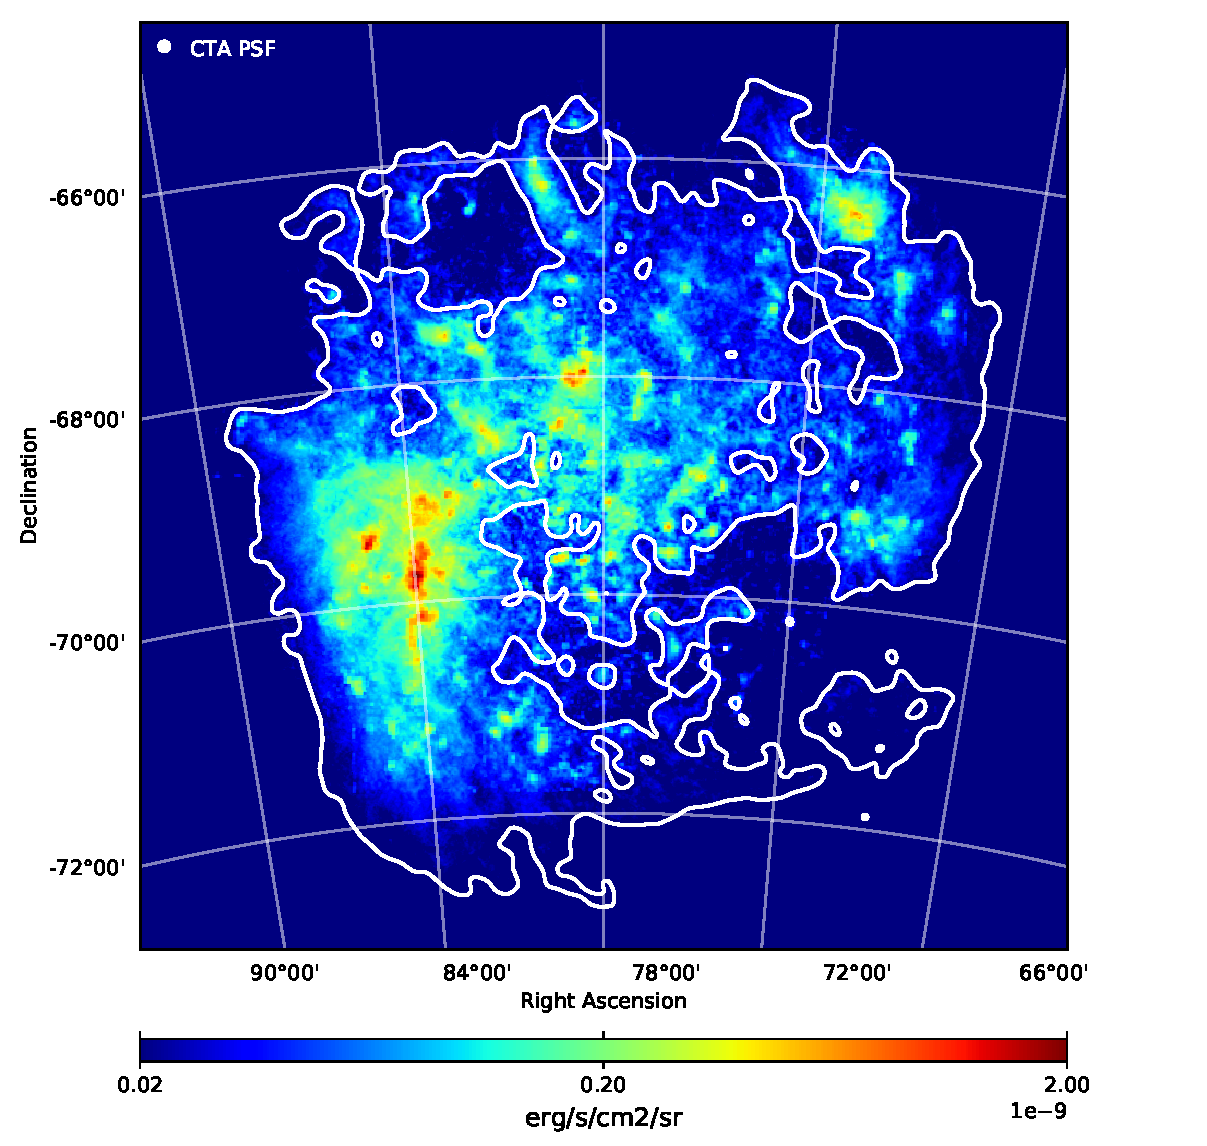
\includegraphics[width=1\textwidth]{Pictures/LMC-Pion_map-1TeV.pdf}
\endminipage 
\minipage{0.5\textwidth}
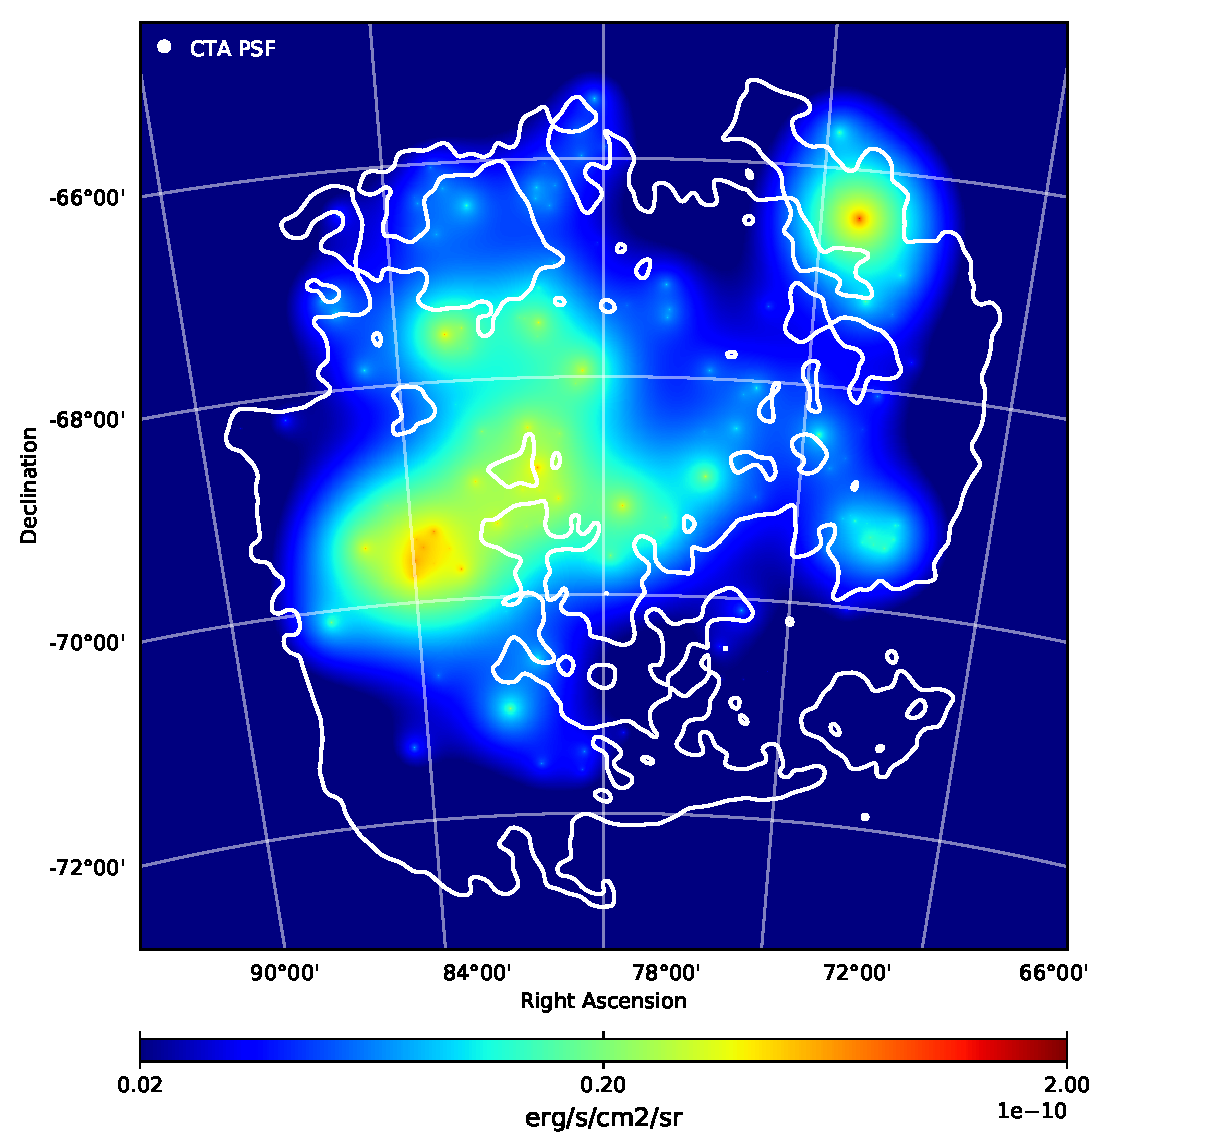
\includegraphics[width=1\textwidth]{Pictures/LMC-IC_map-1TeV.pdf}
\endminipage \\
  \caption{Intensity maps at 1 TeV for large-scale interstellar emission in the \gls{lmc} computed as described in section \ref{sec:diffusemodel}. \textit{Left}: Pion-decay diffuse emission. \textit{Right}: \gls{ic} diffuse emission. White contours trace the extent of the most of the gas disk.}
    \label{fig:mapmodels_cr}
\end{figure}

\subsection{Point Sources}\label{sec:point}

Observations in $\gamma$-rays of the \gls{lmc} have provided a catalog of powerful point-like sources of different nature, which have revealed very interesting features. For this work, we use the \gls{lmc} data collected by \textit{Fermi}-LAT \cite{2010FermiLATLMC11months} \cite{2016LMCFermiLAT} and \gls{hess} \cite{2012HESSLMC} \cite{2015HESSTeVLMC} \cite{2017HESSLMCP3} to build the emission models of the sources included in this study. A description of the different point sources and their emission models is given in the next subsections.

\subsubsection{Pulsar Wind Nebula N157B}

A signal of $\gamma$-ray emission from the direction of the \gls{pwn} N 157B associated to the pulsar  PSR J053-6910 has been measured both by \textit{Fermi}-LAT in the \gls{he} range ($\sim 10 \sigma$) and by \gls{hess} in the \gls{vhe} range ($33 \sigma$). This is the first and only \gls{pwn} ever detected outside the \gls{mw} in $\gamma$-rays \cite{2012HESSN157B}. \gls{pwne} are the result of a supernova explosion, where a fast-rotating, highly-magnetized central pulsar powers a nebula of ultra-relativistic particles with its spin-down energy, i.e. the loss rate of rotational energy. The well known Crab \gls{pwn} is an object of this kind, which seems to present large similarities with N157B. The central pulsar of this system, PSR J053-6910 was first discovered in X-ray energies and seems to be the most powerful pulsar known, with a spin-down power of $\Delta E = 4.9 \cdot 10^{34} $ erg s$^{-1}$ \cite{1998PulsarN157B}. The TeV $\gamma$-ray emission of this kind of objects is directly connected to their spin-down power and has its origin in the \gls{ic} scattering of lower energy photons by relativistic electrons (and positrons). Thanks to its extremely high power, the emission from N157B can be detected despite its large distance ($\sim 48 kpc$ \cite{2006N157Bdistance}) because it is embedded in the strong infrared photon-fields from nearby sources of the superbubble formed by the stellar association LH99, which serve as additional targets for \gls{ic} scattering.
To model this source, we follow the results from \cite{2015HESSTeVLMC}, where the multiwavelength data (X-rays from Chandra \cite{2001ChandraN157B} and $\gamma$-rays from \textit{Fermi}-LAT and \gls{hess}) can only be explained with a leptonic \gls{ic} model where the highest possible magnetic field should be 45$\mu$ G. The  spectral model adopted for this source is shown in figure \ref{fig:PS}.

\begin{figure}[h]
  \centering
  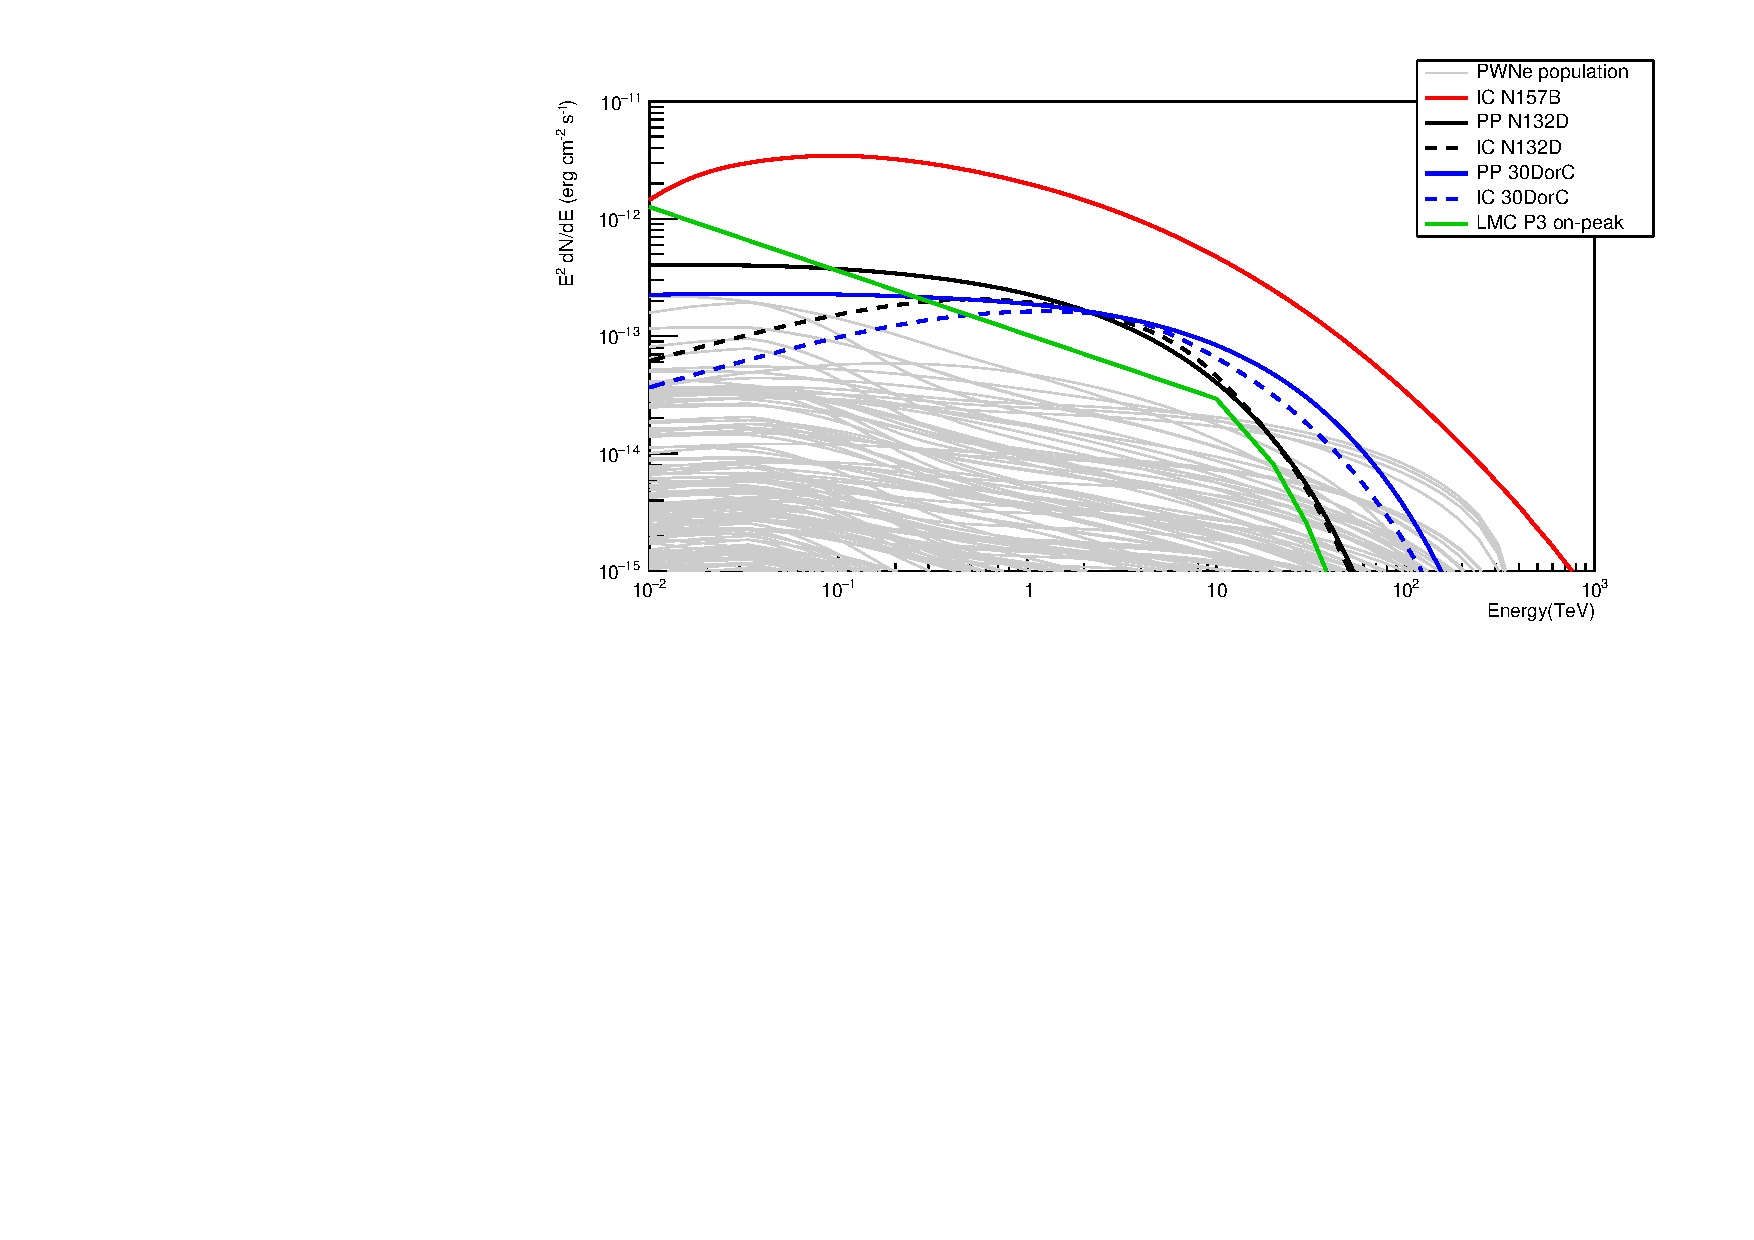
\includegraphics[width=\textwidth]{Pictures/pointsourcesspec.pdf}
  \caption{\label{fig:PS} Spectral energy distribution of the point sources in the \gls{lmc}. Spectra from N157B, N132D and 30DorC are extracted from \cite{2015HESSTeVLMC}. Spectrum of LMC P3 is a power-law with the spectral parameters of the on-peak orbital region from \cite{2017HESSLMCP3}, with an exponential cut-off at 10 TeV. Spectra from the \gls{pwne} population are derived following the baseline model described in section \ref{sec:pwnepop}}
\end{figure}

\subsubsection{Supernova Remnant N132D}

Both \textit{Fermi}-LAT and \gls{hess} have detected $\gamma$-ray emission with strong evidences to belong to the \gls{snr} N132D, a very bright thermal X-ray remnant. It is the brightest remnant of the \gls{lmc} and belongs to a rare type of oxygen-rich remnants which show optical emission from pure heavy-element ejecta, similar to the \gls{mw} \gls{snr} Cas A \cite{2007N132D}. The origin of this \gls{snr}, deduced by its chemical composition, is the core-collapse supernova of a massive progenitor star of mass $> 35 M_{\odot}$ \cite{2007N132D}. The origin of the $\gamma$-ray emission yields on the interaction of the supernova shock with the cloud of dense material ejected by the progenitor star during its lifetime. The flux detected by \gls{hess} \cite{2015HESSTeVLMC}, with a $\gamma$-ray luminosity in the 1-10 TeV band of $0.9 \pm 0.2 \times 10^{35}(d/50kpc)^2$ erg/s, allows to consider the possibility of two origins of the radiation: In the hadronic scenario the flux of $\gamma$-rays is produced by the decay of neutral-pions, which would imply a remarkably high fraction of energy injected to \glspl{cr} by the supernova explosion, or a gas density higher than the one expected from X-ray observations. Either possibility is plausible given the observations in the optical and infrared bands, which reveals a structure produced by the interaction of the remnant with shocked interstellar gas \cite{2006shockn132D}. In the leptonic scenario, $\gamma$-rays are produced by \gls{ic} scattering of low energy-photons. This model could be supported by the high synchrotron emission in radio and X-rays, however, it would require a lower magnetic field than the one inferred from radio observations ($20 \mu G$ vs. $40\mu G$). The fluxes and spectral index measured by \textit{Fermi}-LAT in \cite{2016LMCFermiLAT} seem to rule out this model.\\
For this work, we assume the hadronic (PP) model shown in figure \ref{fig:PS} based on \gls{hess} measurements.


\subsubsection{Superbubble 30 Dor C}

The Superbubble 30DorC, detected by \gls{hess} in the \gls{vhe} range, is a radiation emitting shell which stands out in X-rays, being the largest X-ray synchrotron shell known (with a radius of 47pc) \cite{200430dorcxrays}, and also emits radio and optical radiation \cite{1985SNRsintheLMC30dorc}. Its origin seems to be related to the stellar winds and supernovae of the stellar association LH 90 \cite{198430dorLH90}. Both leptonic and hadronic scenario could explain the $\gamma$-ray flux detected by \gls{hess} from this source as discussed in \cite{2015HESSTeVLMC}. The two models are shown in figure \ref{fig:PS}. For this work we tested both models, given that \gls{cta} observations from 100 GeV could be able to set which is the most probable model, thanks to the slope differences up to 1 TeV.

\subsubsection{Binary system LMC P3}

This object was first detected by \textit{Fermi}-LAT at \gls{he} energies in \cite{2016LMCFermiLAT}, but was classified as an unidentified source in the environment of the HII regions NGC 2029/NGC2032. They measured a very soft power-law spectrum (index $\sim 2.8$) but did not notice any variability down to a monthly basis.
Later, emission from this object in the \gls{vhe} range was detected by \gls{hess} \cite{2017HESSLMCP3}. They discovered a variability of 10.3 days period, classifying the object as the first extragalactic $\gamma$-ray binary system. The position of LMC P3 is consistent with a soft X-ray source, with variability in X-ray flux. The radial velocity measured from Balmer absorption lines confirmed that it is very likely a binary system \cite{1981softXraysLMC}, \cite{2012xraybinaryP3}. From optical radial velocity measurements, it is derived that the system must be composed by a neutron star with an O5III star companion \cite{2016P3binary}. $\gamma$-ray binaries are believed to be a brief phase of the evolution of high-mass X-ray binaries, in which the $\gamma$-ray emission dominates the electromagnetic output \cite{1989binaries}.\\
The spectrum of LMC P3 (HESS J0536-675) was fitted by \gls{hess} to a simple power law of the form $\frac{dN}{dE} = \Phi_{1TeV}\left( \frac{E}{1TeV}\right)^{-\Gamma}$ with an on-peak spectral index $\Gamma$ of 2.1, and an off-peak index of 2.4, where on-peak represents the orbit region where most of the $\gamma$-ray radiation is emitted. The detection of the source only achieved enough statistical significance during the on-peak period.\\
For simplicity in this work, we will assume the on-peak spectral parameters of the source without any temporal modulation ($\Gamma=2.1$, $\Phi_{1TeV} = 5 \cdot 10^{-13}cm^{-2}s^{-1}TeV^{-1}$). The justification is that the on-peak orbital phase lasts for $\sim 50$h, which is way below the total observation time assigned to the \gls{lmc} survey. An upper limit for the detection of the off-peak region was also calculated and results are given in section \ref{sec:results}.

\subsection{PWNe population in the LMC}\label{sec:pwnepop}

\gls{pwne} are the predominant class of TeV emitters in our Galaxy, with more than 30 sources detected up to date \cite{2009TeVreview}. If we assume that the same is true for the \gls{lmc}, we can model a typical \gls{pwne} population reproducing the so called \textit{baseline} spectral model, first introduced by \cite{2012PWNemodel} and revised by \cite{2018hessPWNe}. The model is a one-zone, time-dependent model which allows to trace the evolution of \gls{vhe} lepton population and hence, radiative output of a \gls{pwn}.
In the model, the number of leptons with energy $E$ residing in the nebula at time $t+\delta t$ will be determined by the balance between the injected leptons and those cooled out in the respective energy interval:

\begin{equation}
\frac{dN}{dE}(E, t+\delta t) = \frac{dN_{cooled}}{dE}(E,t+\delta t) + \frac{dN_{inj}}{dE} (E, t+\delta t)  
\end{equation}

Where for the number of injected leptons $dN_{inj}/dE$ a power-law spectral shape is assumed:

\begin{equation}
  \frac{dN_{inj}}{dE}(E,t) = \Phi_{0}(t) \left(\frac{e}{1 TeV} \right)^{-\beta}
\end{equation}

with a power-law index $\beta$, also known as injection index. The normalization $\Phi_0(t)$ will depend on the amount of spin-down energy converted into relativistic electrons and positrons in a time step $t+\delta t$.
The cooling mechanisms comprise synchrotron escape and adiabatic losses, and the number of cooled leptons can be approximated by:

\begin{equation}
  \frac{dN_{cooled}}{dE}(E, t) = \frac{dN}{dE} (E, t-\delta t)\cdot exp \left(-\frac{\delta t}{\tau_{eff}(E,t)} \right)
\end{equation}

Where $\tau_{eff}$ is the effective cooling timescale, which will depend on the time evolution of the \gls{pwn} radius and magnetic field strength.\\
The baseline model requires a series of parameters which are listed in table \ref{tab:baselinemodelpwne}:

\begin{table}
  \centering
  \begin{tabular}{llll}
    \hline
    Parameter description & & & Parameter values \\
    \hline
    Braking index & n &  & 3.0 \\
    Initial spin-down power & $\dot E_{0}$ & ($10^{39}$ erg s$^{-1}$) & 2.0 \\
    Initial spin-down timescale &$\tau_{0}$ & (kyr) & 0.5 \\
    Initial magnetic field strength & $B_{0}$ & ($\mu$ G) & 200\\
    Reverse shock interaction timescale & $\tau_{rs}$ & (kyr) & 4.0 \\
    \gls{pwn} radius at t=3kyr & $R_{3}$ & (pc) & 6.0 \\
    Adopted const. \gls{ism} magn. field strength & $B_{ISM}$ &($\mu$ G) & 3.0 \\
    Lepton conversion efficiency & $\eta$ & & 1.0 \\
    Index of magnetic field evolution & $\alpha$ & & 0.6 \\
    Index of letpon injection spectrum & $\beta$ & & 1.75, 2.0, 2.25\\
    Lower bound of lepton energy distribution & $E_{min}$ & (TeV) & 0.03 \\
    Upper bound of lepton energy distribution & $E_{max}$ & (TeV) & 300\\
    \hline
  \end{tabular}
  \caption{Parameters used for the modelling of the \gls{pwne} population, based on table A.1 from \cite{2018hessPWNe}.}
  \label{tab:baselinemodelpwne}
\end{table}

Three equally probable values of the injection index $\beta$ have been considered, and the interstellar magnetic and radiation fields have been adapted to the average conditions in the \gls{lmc}.\\
The population of \gls{pwn} has been generated considering that pulsars are born at a rate of $r_{CC} = 0.0011 SN yr^{-1}$, in agreement with the assumed rate of \gls{sne} explosion and ratio of core-collapse to thermonuclear \gls{sne}, assuming that all core-collapse \gls{sne} lead to the formation of a spinning neutron star. The lifetime for each \gls{pwn} is approximated as of $\tau_{PWN} = 200 kyr$, which yields to an average number of $r_{CC} \times \tau_{PWN} = 220$ \gls{pwne} in the \gls{lmc} if the pulsar creation is in steady state during the time $\tau_{PWN}$. The following steps have been carried on to generate the synthetic population of \gls{pwne}:

\begin{itemize}
\item (i) Draw a random number of objects from a Poisson distribution with mean $r_{CC} \times \tau_{PWN}$.
\item (ii) Draw random ages from a uniform distribution over 0 to $\tau_{PWN}$.
\item(iii) Random select an injection index among the three values considered, listed in table \ref{tab:baselinemodelpwne}.
\item (iv) From the baseline spectral model, compute the spectra of all objects given their ages and injection indices.
\item (v) Distribute them spatially among the different massive star forming regions, in proportion to their ionizing luminosity.
\item(vi) Add some luminosity scatter to reflect the properties of the observed \gls{pwne} population in the \gls{mw}.
  \item(vii) Apply two cuts in the synthetic population: First, remove objects younger than 2kyr, because we already know at least two objects of that age (SN 1987A and N158A); second, remove all objects with > 1TeV luminosity above $2.2 \times 10^{34}$ erg s$^{-1}$, because they would have been detected by \gls{hess} already, as shown in the upper limits calculated for SN1987A in \cite{2012HESSLMC}. 
\end{itemize}

The total number of 189 \gls{pwne} have been included in the simulated model, and their spectral energy distributions are shown in figure \ref{fig:PS}. A mapcube of the emission of the \gls{pwne} population at 1 TeV is shown in picture \ref{fig:mapcube_pwne}.


\begin{figure}[h!]
  \centering
  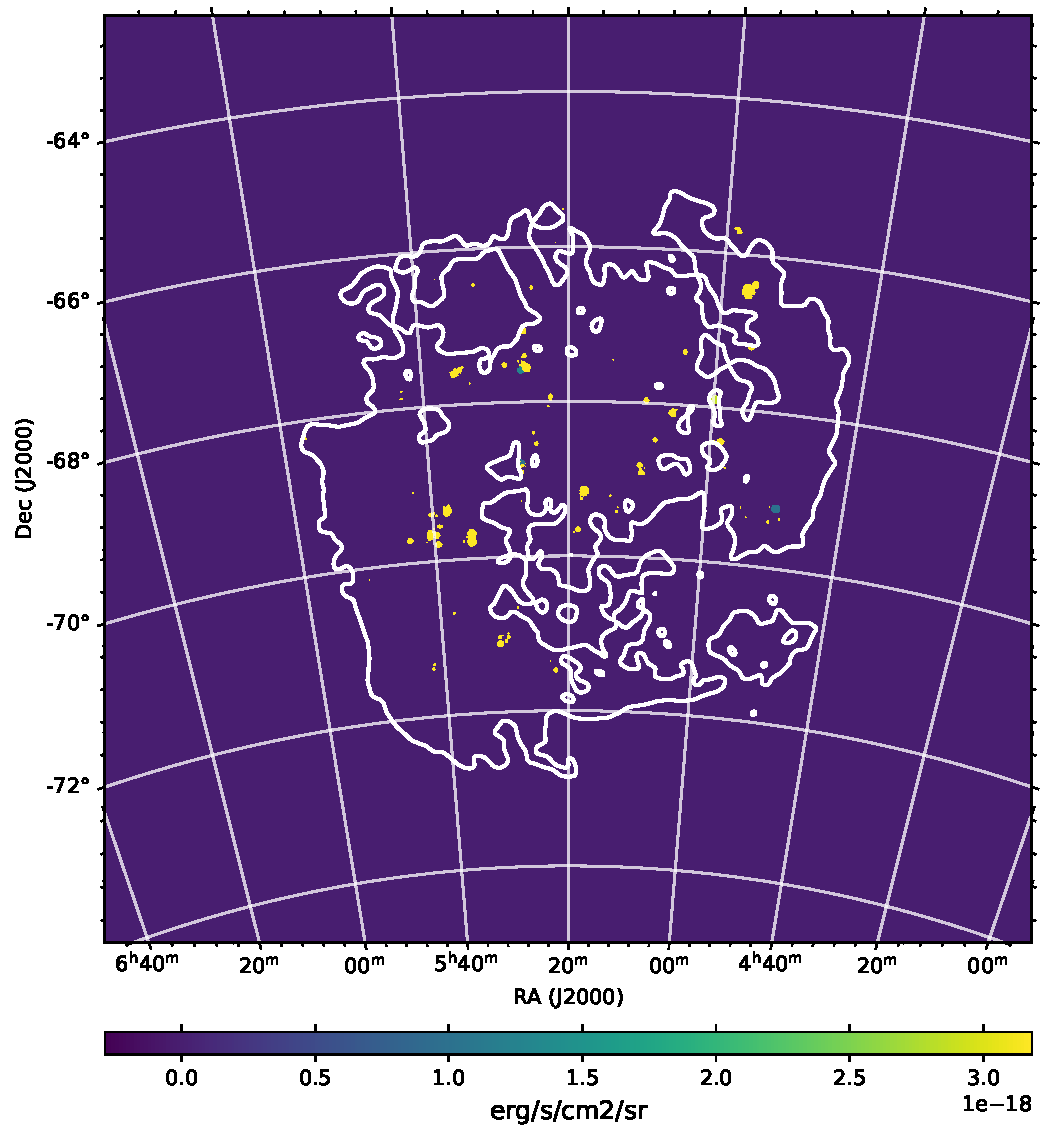
\includegraphics[width=0.4\textwidth]{Pictures/PWNe_1TeVmap.pdf}
  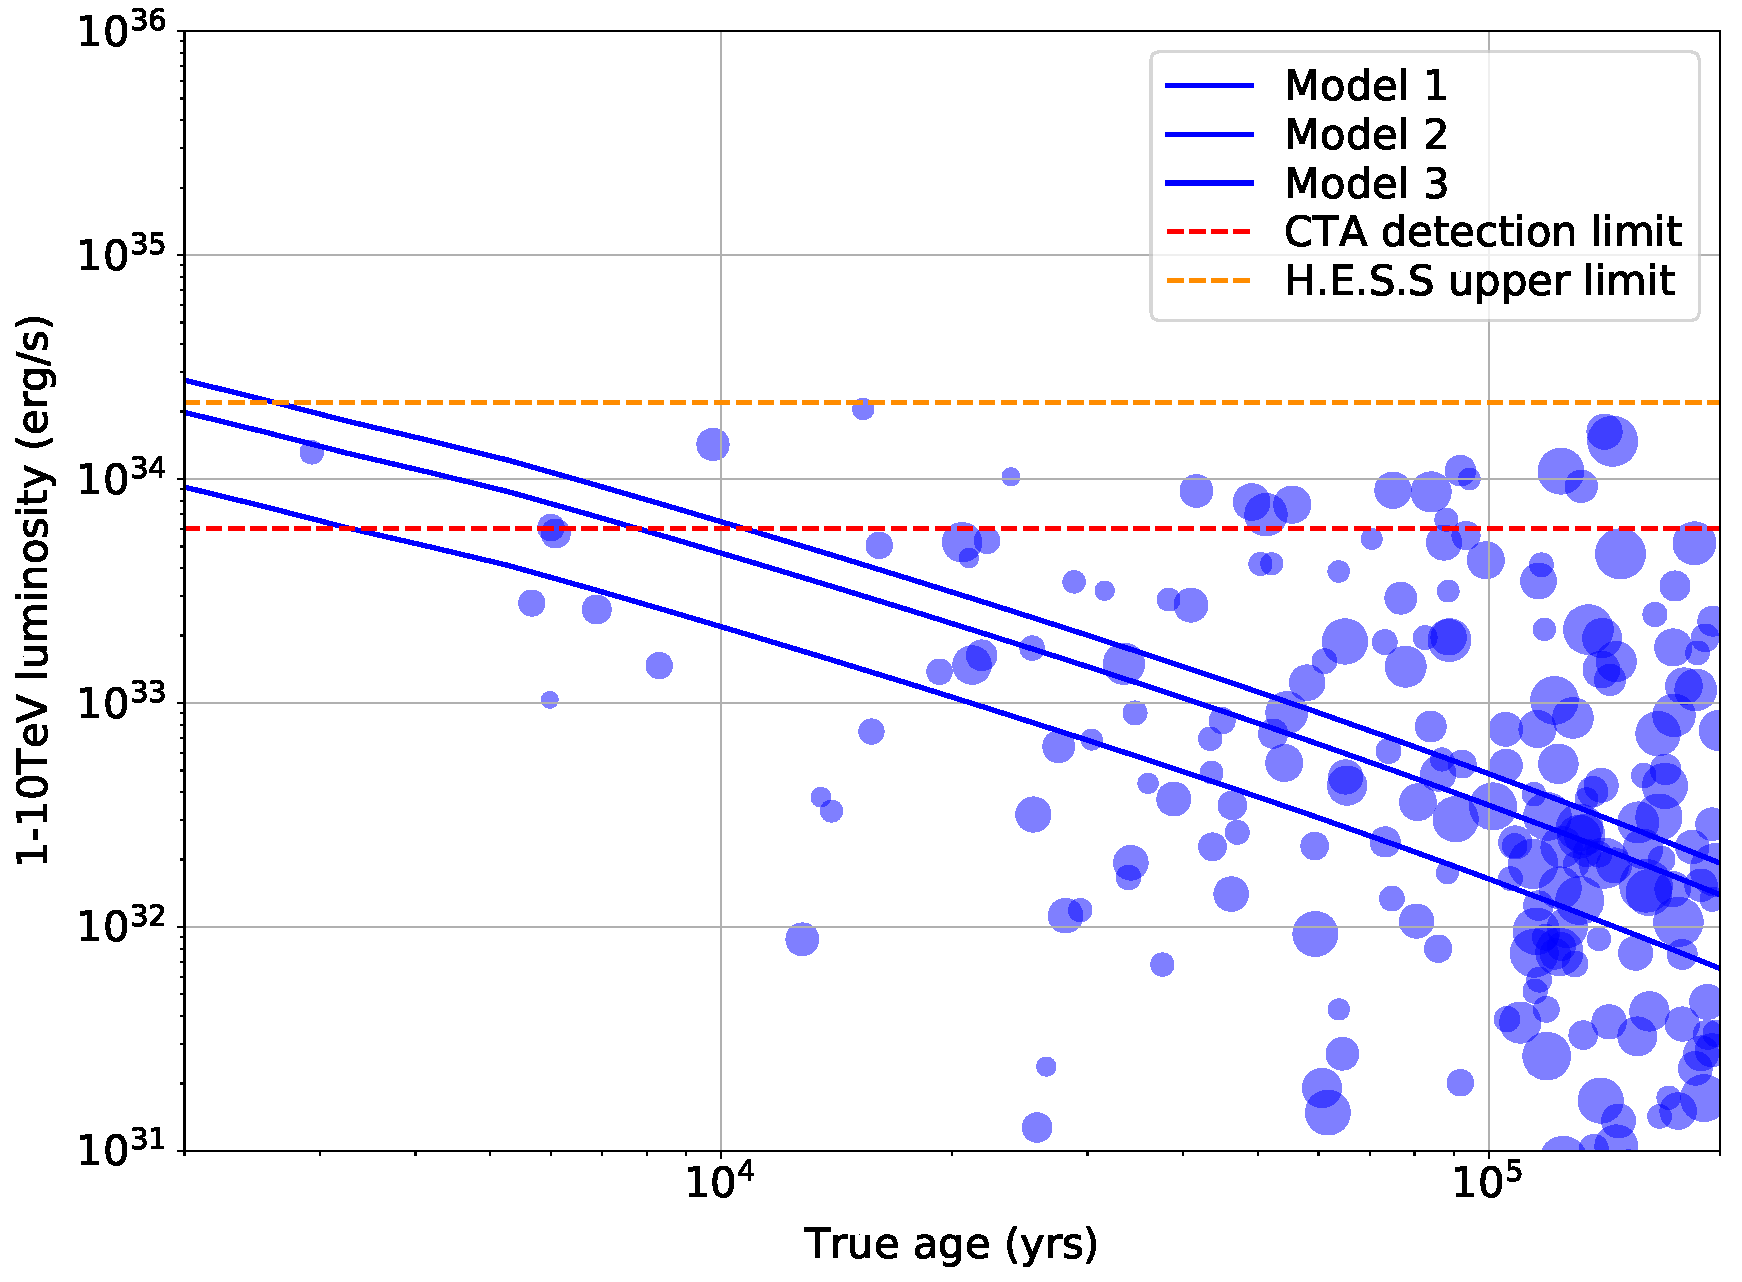
\includegraphics[width=0.55\textwidth]{Pictures/LMC-PWNe_lum-vs-age.pdf}
  \caption{ \textit{Left}: Mapcube of the \gls{pwne} synthetic population generated as described in section \ref{sec:pwnepop} at 1 TeV. \textit{Right}: Luminosity as a function of age for one random sample of our \gls{pwne} population model. Dot size is linearly proportional to \gls{pwn} radius. Overlaid are the average relations for the different models from which the population was drawn (models 1 to 3, differing by the particle injection index, from 1.75 to 2.25), the upper limit on point-like emission from H.E.S.S. \cite[using the limit on SN1987A from][]{Abramowski:2015}, and the threshold for detection with \gls{cta}.}
  \label{fig:mapcube_pwne}
\end{figure}

\section{Simulations and Analysis method} \label{sec:simana}

\subsection{Region of Interest and Observational strategy}

The  \gls{roi} of the \gls{lmc} extends about 10º in the sky. In order to reach this large \gls{fov}, \gls{cta} will cover the full region by a series of slightly overlapping pointings with a \gls{fov} of $\sim 3º$ each. The total amount of hours assigned to the \gls{lmc} survey is 340h plus 150h more in case the \gls{snr} 1987A is detected. For this work, different pointing patterns have been tested in order to adopt the observational strategy which will maximize the significance of detection both for point sources and extended sources. The final scheme consist on 7 pointings arranged in 3 rows with a 2-3-2 configuration centered in the coordinates RA=80.0º, dec=-69.0º with a separation of 2º between pointings, as shown in figure \ref{fig:pointings}. The duration of the observation in each pointing position is of $\sim 1.75 \times 10^5$ s. For the simulations performed in this work, all telescopes planned for \gls{cta} South are involved. 

\begin{figure}[h]
  \centering
  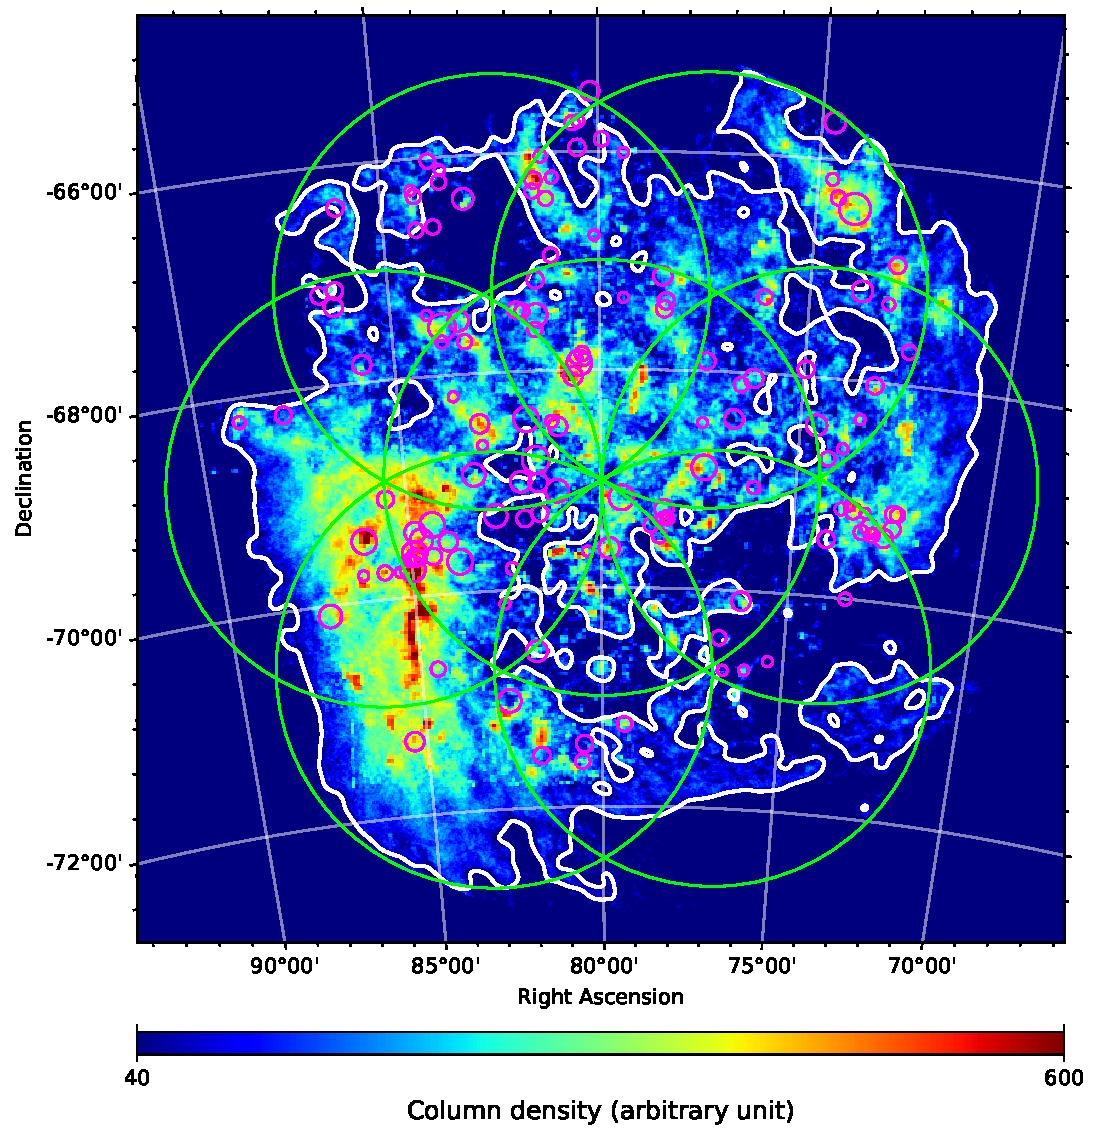
\includegraphics[width=0.7\textwidth]{Pictures/map_pointings_data.pdf}
  \caption{\label{fig:pointings} Total hydrogen gas column denisty map in the the region of interest of the \gls{lmc}. The pointing pattern is overlapped in the shape of green circles. Magenta circles give the position of the HII regions selected as \gls{cr} injection sites, with circle size proportional to the logarithm of the ionizng luminosity, used as proxy for relative \gls{cr} injection power.}
\end{figure}

\subsection{Simulation parameters}

To calculate the predicted number of counts from a certain emission model, the \gls{cta} collaboration provides a set of \glspl{irf} \cite{CTAPerformance} with information about the effective area and angular resolution of the instrument for several zenith angles. For this work we have used the \gls{irf} \textit{South\_z40\_50h} from the production \textit{prod3b-v2}. This \gls{irf} only accounts for the southern observatory and is optimized for zenith angles around 40º (\gls{lmc} will be observed at $\sim 46$º from the southern site) and 50 hours of observation time. \\
The simulations were computed using \textit{ctools} and \textit{gammalib} \cite{2016Actools}, a software framework for the analysis of astronomical $\gamma$-ray data, specifically designed for \gls{cta} (see section \ref{sec:ctools}). The function \textit{ctobssim} uses a \gls{mc} generator to recreate event lists for observations. As input, it requires a full model of the \gls{roi}, including each individual source with a spatial and spectral component, and a model of the instrumental background accounting for \gls{cr} events misidentified as $\gamma$s.
Also, \textit{ctobssim} requires the \gls{irf} for the observation and the energy range. Each running of \textit{ctobssim} results in a realization of the model where the event list is generated with a random number generator. We have performed realizations of the full emission model of the \gls{lmc} with the pointing pattern described before, in the energy range from 0.05 TeV to 150 TeV. \textit{Ctobssim} is able to combine the different observations of the overlapping pointings, averaging the \glspl{irf} of each region. The resulting event lists are written into FITS files, one for each pointing, which can be combined afterwards for the analysis.\\

\subsection{Fitting method}

A binned likelihood analysis has been performed in this work, to fit the emission model to the simulated data. The event lists of the 7 pointings have been combined and then the data has been binned into 110 energy bins using the \textit{ctools} function \textit{ctbin}. The boundaries of the energy bins have been generated using the function \textit{csebin}, which inspects the variation in the effective area and background template of the \gls{irf} with energy, for the specific simulations. It settles a bin boundary when the quantities change in a fraction selected by the user. To ensure a sufficiently large number of energy bins (it is recommended to have at least 30 bins per decade), the threshold for the fractional change in effective area has been settled to 0.06, and to 0.16 for background rate. \\
The energy range chosen for the analysis is from 100 GeV to 100 TeV. The higher lower limit, compared to the full range of \gls{cta} (which can go down to 30 GeV) comes from the limitations of performance at high zenith angles, given that \gls{lmc} will be always observed at z > 40º.
The background model, the exposure cube and point spread function cube are precomputed using the functions \textit{ctbkgcube}, \textit{ctexpcube} and \textit{ctpsfcube} respectively. The results are a series of mapcubes which will be used to calculate the maximum likelihood function.\\
An Asimov data set has been computed to produce the results presented in this chapter. The \textit{Asimov} data set \cite{2011Asimov} is a representative data set which, when fitted, will retrieve the true values of the model parameters. It can be computed with \textit{ctools} using the function \textit{ctmodel}, and allow to give mean results for significance and upper limits without needing a large number of realizations of the simulated data.\\
Different slices of the Asimov dataset produced for this analysis is shown in picture \ref{fig:asimov}. 

\begin{figure}[h!]
  \centering
  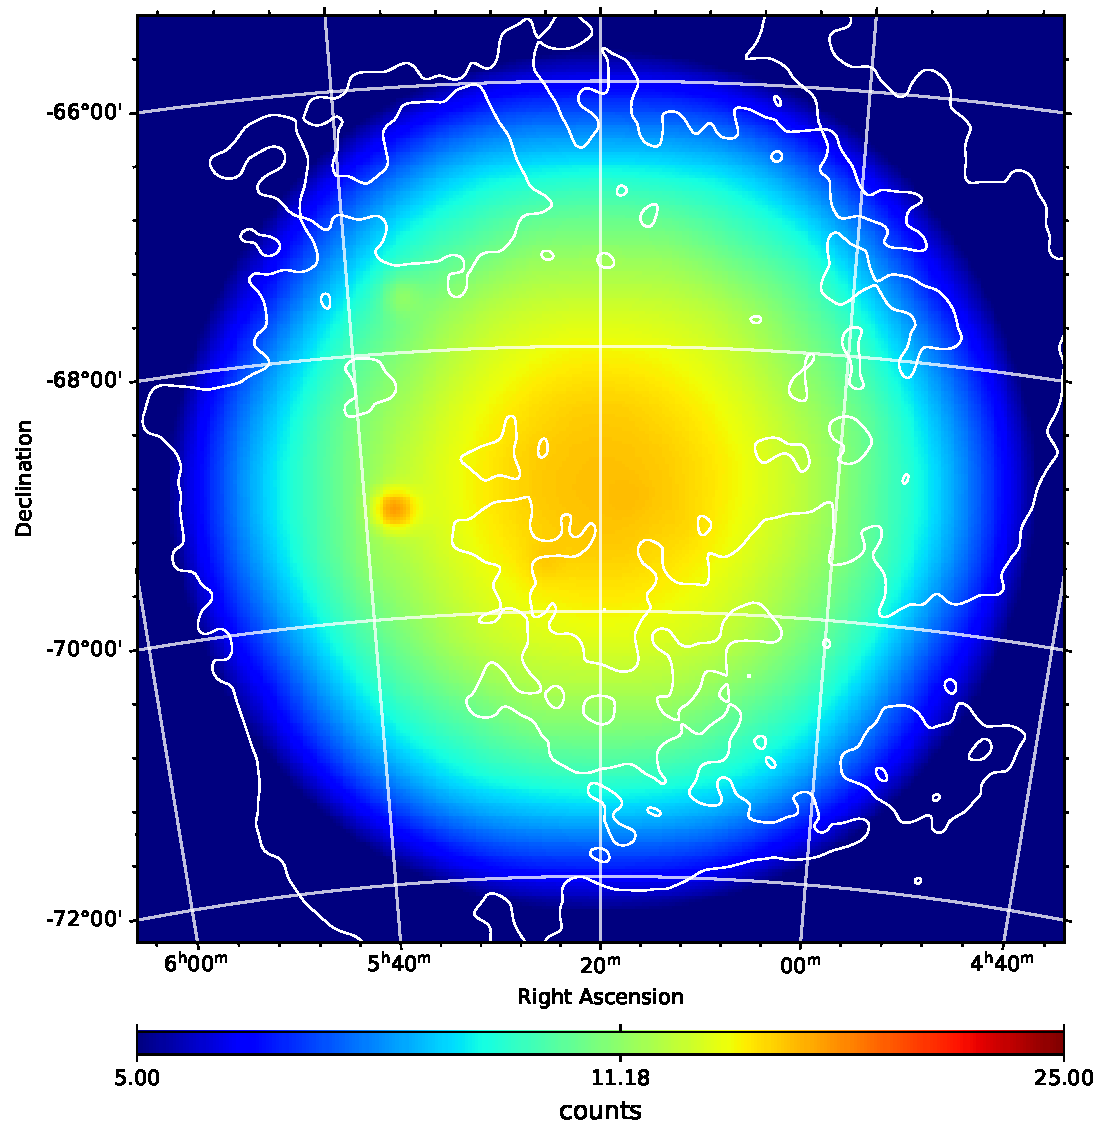
\includegraphics[width=0.32\textwidth]{{Pictures/Asimov_0.100-0.105_TeVmap}.pdf}
  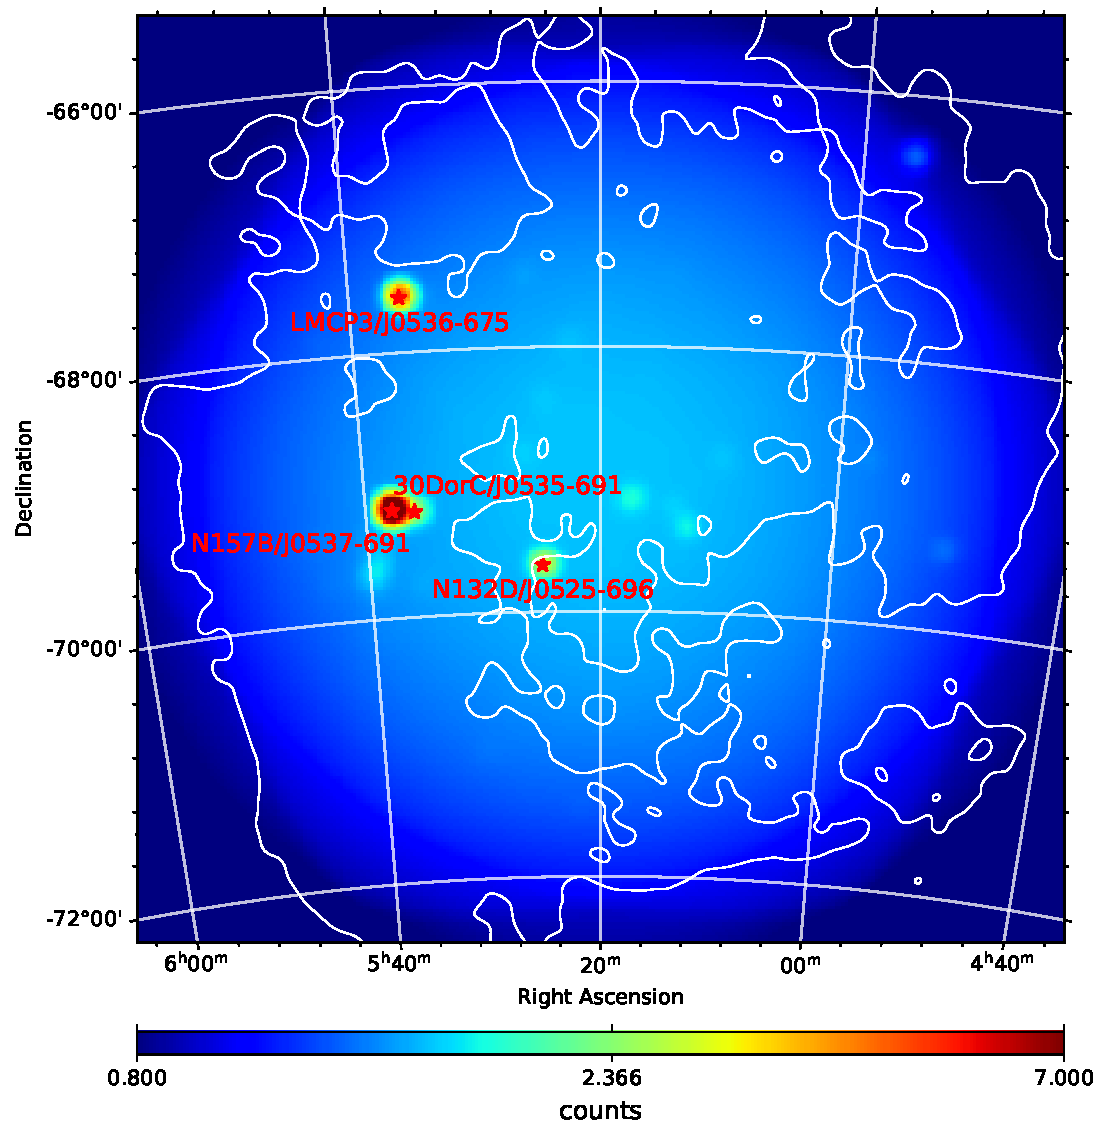
\includegraphics[width=0.32\textwidth]{{Pictures/Asimov_0.975-1.040_TeVmap}.pdf}
  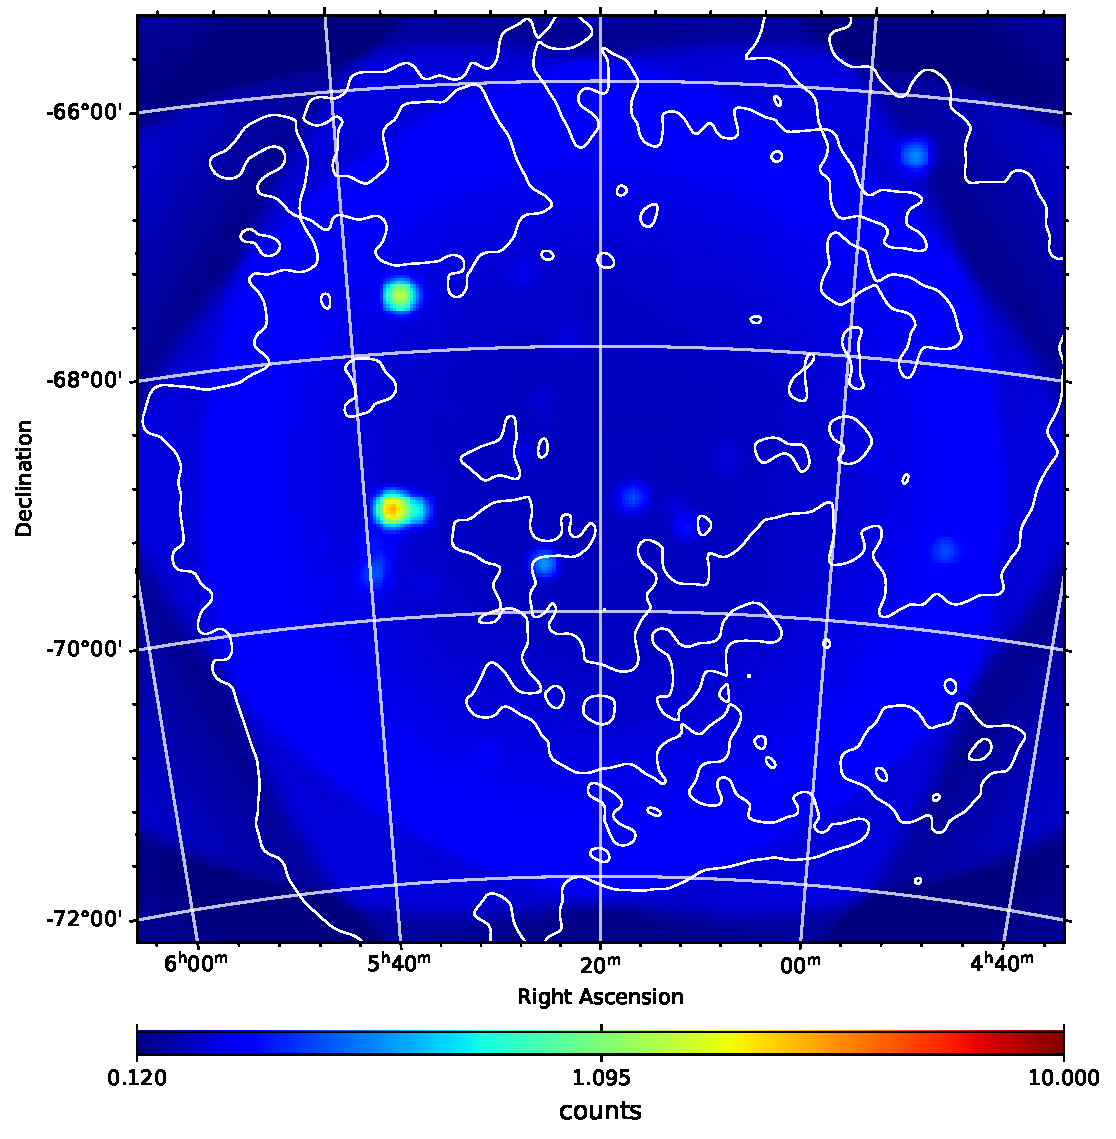
\includegraphics[width=0.32\textwidth]{{Pictures/Asimov_8.858-10.055_TeVmap}.pdf}
  \caption{\label{fig:asimov} Three slices of the Asimov mapcube at 0.100 TeV, 1 TeV and 10 TeV ( \textit{left}, \textit{middle},  and \textit{right} respectively) produced with the full emission model of the \gls{lmc} described in section \ref{sec:model}. The four H.E.S.S. point sources are marked with red stars in the 1 TeV map.}
  \end{figure}

\subsubsection{3D Likelihood Analysis for $\gamma$-ray sources}

The likelihood analysis is based in the Poisson likelihood function:
\begin{equation}
  \mathcal{L}(\mu | n) = \prod_{i,j}\frac{\mu_{ij}^{n_{ij}}}{n_{ij}!}e^{-\mu_{ij}}
  \label{eq:likelihood}
\end{equation}

Where $n_{ij}$ represents the simulated counts and $\mu_{ij}$ the model prediction for each bin in energy(i) and space (j). The model $\mu_{ij}$ is the result of the combination of the models for each of the $\gamma$-ray sources described in section \ref{sec:model}. Each source model accounts for a spectral and a spatial component. For extended sources, both components are combined in one mapcube. In the likelihood fitting the only free parameter for each of these models is the spectral normalization $A^{X}$, which determine the relative weight of component $X$. The only exception is the point source LMC P3, which spectral model is a power-law where the free parameters are the normalization and the spectral index. The shape of $\mu$ is therefore:

\begin{equation}
  \mu_{ij}(A^{X}) = \sum_{X} A^{X} \mu^{X}_{ij} + A^{LMC P3}(E)^{-\Gamma}
\end{equation}

The maximum likelihood is calculated finding the normalization parameters $A^{X}$ which maximize equation \ref{eq:likelihood}.\\
The detection significance of a source is calculated in terms of the Test Statistics:

\begin{equation}
  TS = 2log \frac{\mathcal{L}(\mu(A^{X})|n)}{\mathcal{L}_{null}}
  \label{eq:ts}
\end{equation}

Where $\mathcal{L}(\mu(A^{X})|n)$ is the maximum likelihood function and $\mathcal{L}_{null}$ is the value of the likelihood function of the null hypothesis for the specific source (meaning $A^X$ = 0). With this definition, typically a source is considered to be detected when $TS>25$, equivalent to $5\sigma$.\\
The maximum likelihood analysis has been performed using the function \textit{ctlike} from \textit{ctools}. The inputs are the data mapcubes from the stacked analysis and the description of the emission model. For the likelihood fit the same emission model used for the simulations is given as input, meaning that the fitting results will represent the most optimistic case, where the model is perfectly describing the data. 

\subsubsection{Upper limits calculation} \label{sec:ulimits}

For sources which have a flux too low to be detected ($TS < 25$) we calculate upper limits on the minimum flux needed for the source to be detected with \gls{cta}. We calculate this upper limits as the flux that leads to a decrease in the likelihood that corresponds to a certain \gls{cl}. This is the chosen definition for upper limits in this work, as it is the one included in \textit{ctools}, but it must be noted that other definitions exist in the literature.
Using the definition of TS from \ref{eq:ts}, according to Wilks' theorem \cite{wilks1938}, the TS function asymptotically approaches a $\chi^2$-distribution with one degree of freedom under the null hypothesis, therefore to get the flux that yields to the 95\% \gls{cl} upper limit, we must find the normalization parameter $A^X_{max} > A^{X}$ which corresponds to TS = 2.71.\\
This calculation is performed using the function \textit{ctulimit} from \textit{ctools}, which requires as input the mapcube of the simulated data and a model with all the sources, including the source for which the upper limit will be calculated. In this case, we use the model resulting from the maximum likelihood fit. The only free parameters must be again the spectral normalizations. The results from \textit{ctulimit} are the upper limit in the differential flux for a reference energy, the integrated upper flux limit for a specific energy range and the integrated upper energy flux limit for the same range.\\
We have used this method to set constraints on the \gls{dm} annihilation cross section $<\sigma v>$ as described in section \ref{sec:dminlmc}.

\section{Results}\label{sec:results}
        
\subsection{Point sources}

The results for the fitting of the four point sources tested in this work in the full energy range (100 GeV to 100 TeV) are given in table \ref{tab:fitsources}. The significance of detection of the sources is given in terms of the Test Statistics described in the previous section. For LMC P3 three cases have been tested: The case of a spectrum following a power-law with the on-peak parameters from \cite{2017HESSLMCP3}; the same power-law but with an exponential cut-off at 10 TeV; and a last case where no source has been simulated, but an upper limit on the flux for a source with the off-peak spectral index has been computed in the energy range 0.1-100 TeV. Also, energy flux upper limits for three energy ranges are shown in figure \ref{fig:sensiulimits}.\\
The results show that \gls{cta} will be able to detect with high significance all the known point sources in the \gls{lmc}, including the binary system \gls{lmc} during the on-peak orbital region, and will be able to test the flux of the off-peak region. 

\begin{table}
  \centering
  \resizebox{\textwidth}{!}{%
  \begin{tabular}{llllll}
    \hline
    Source name & RA(º) & Dec(º) & Normalization & TS & Significance($\sigma$) \\
     &  &  & $(0.1 - 100 TeV)$ &  &  \\
    \hline
    & & Point Sources & & & \\
    \hline
    N157B/HESS J0537-691 & 84.44 & -69.18 & $1\pm 0.005$ & 130951.51 & 361.9 \\
    N132D/HESS J0525-696 & 81.26 & -69.64 & $1\pm 0.019$ & 5370.19 & 73.3\\
    30DorC/HESS J0535-691 (PP) & 83.96 & -69.2 & $0.999 \pm 0.022$ & 4762.83 & 69.0 \\
    30DorC/HESS J0535-691 (IC) & 83.96 & -69.2 & $0.999 \pm 0.022$ & 3919.0 & 62.6 \\
    LMCP3/HESS J0536-675 & 84.0 & -67.59 & Prefactor: $4.99\pm0.05 \cdot 10^{-19}$ & 27353.83 & 165.4 \\
    (on-peak, cut-off 10 TeV) &  &  & $(cm^{-2}s^{-1}MeV^{-1})$ &  &  \\
    & &  & Index: $2.1 \pm 0.01 $ &  &  \\
    LMCP3/HESS J0536-675 & 84.0 & -67.59 & Prefactor: $4.99\pm0.05 \cdot 10^{-19}$ & 48021.95 & 219.14 \\
    (on-peak)&  &  & $(cm^{-2}s^{-1}MeV^{-1})$ &  &  \\
    & &  & Index: $2.1 \pm 0.006 $ &  &  \\
    LMCP3/HESS J0536-675 & 84.0 & -67.59 & Int. flux ulimit (99 \% CL): $1.23 \cdot 10^{-13}$ & - & - \\
    (off-peak)&  &  & $(cm^{-2}s^{-1})$ &  &  \\
    \hline
    & & Diffuse emission components & & & \\
    \hline
    LMC Pion-decay & - & - & $1\pm0.185$ & 29.06 & 5.39 \\
    LMC IC & - & - & Int. flux ulimit(99\% CL): $7.33 \cdot 10^{-12}$ & - & - \\
     &  &  & $(cm^{-2}s^{-1})$ &  &  \\
    
    \hline
  \end{tabular}}
  \caption{Results of the fit for the point sources and diffuse components included in the emission model. For the first three sources, the normalization of the spectrum is the only free parameter to fit. For LMCP3, a power-law spectrum with exponential cut-off at 10 TeV has been fitted, accordingly with the results of \cite{2017HESSLMCP3}. For the off-peak region, the upper limit at 99\% \gls{cl} for the integrated flux has been calculated. From the diffuse components, only the hadronic emission could be detected at $TS>25$ therefore an upper limit has been computed for the leptonic \gls{ic} component.}
  \label{tab:fitsources}
\end{table}

\subsection{Population of PWNe}

For the fitting of the \gls{pwne} population, a mapcube including all the artificially computed candidates has been used for simulation. Then, each \gls{pwn} spectrum has been fitted individually, keeping all the rest of the \gls{pwne} and other model components fixed. The results show that 15 from the total of 189 simulated \gls{pwne} would be detected with $TS>25$, giving an estimation of the number of new \gls{pwne} that could be discovered by \gls{cta}. Also, 12 more \gls{pwne} were fitted giving a $TS>9$ ($3\sigma$ significance). It must be taken into account that this is a very optimistic result, giving that the true spectrum and position of each \gls{pwne} is being used for fitting. In reality, a totally blind search will be performed, scanning the full region in the search for excesses, and assuming a generic spectral shape. The results on the \gls{pwne} are shown in figure \ref{fig:pwnepopresults}, showing the fitted flux compared to the true flux, and the TS value vs. the true flux.

\begin{figure}[h!]
\centering
\minipage{0.5\textwidth}
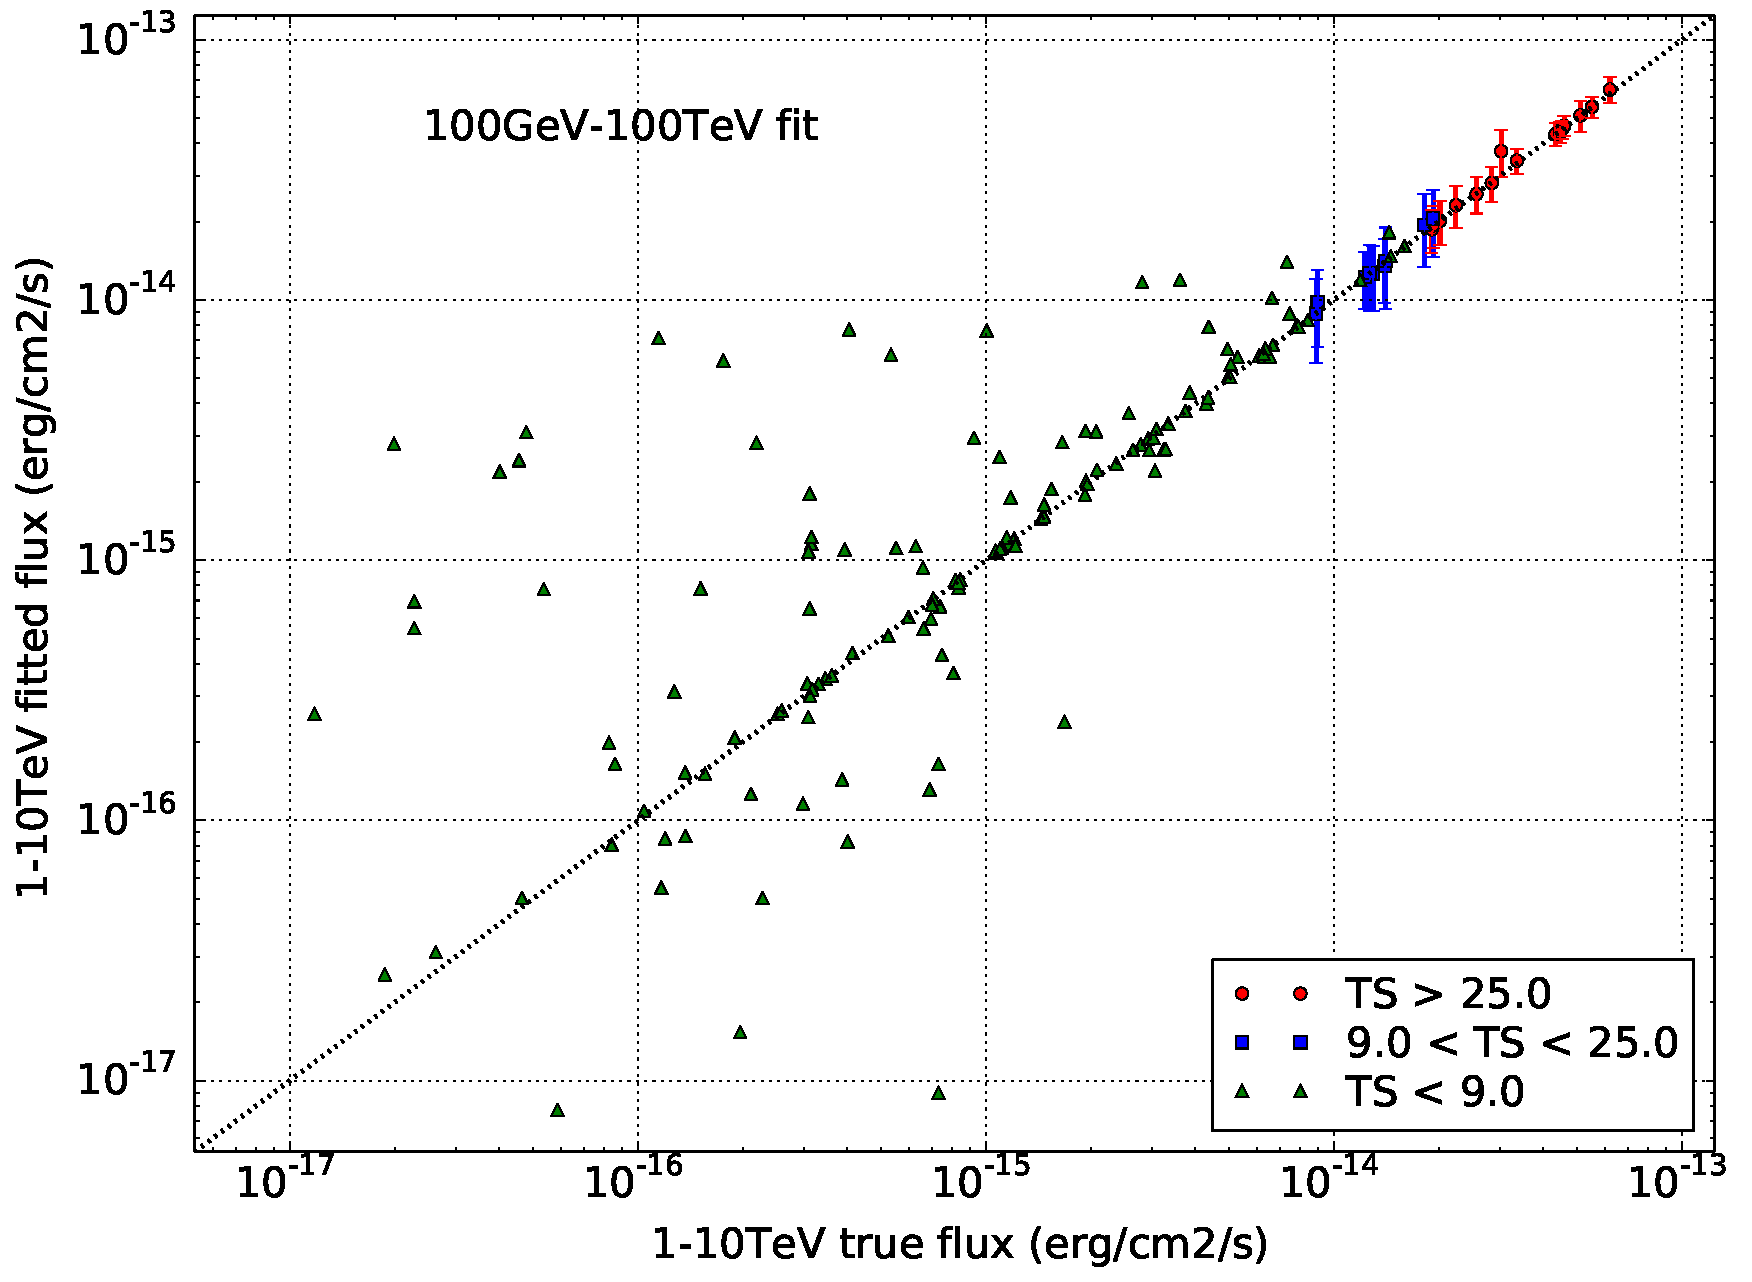
\includegraphics[width=1\textwidth]{Pictures/PWNe-only_Flux_100GeV-100TeV_Asimov.pdf}
\endminipage 
\minipage{0.5\textwidth}
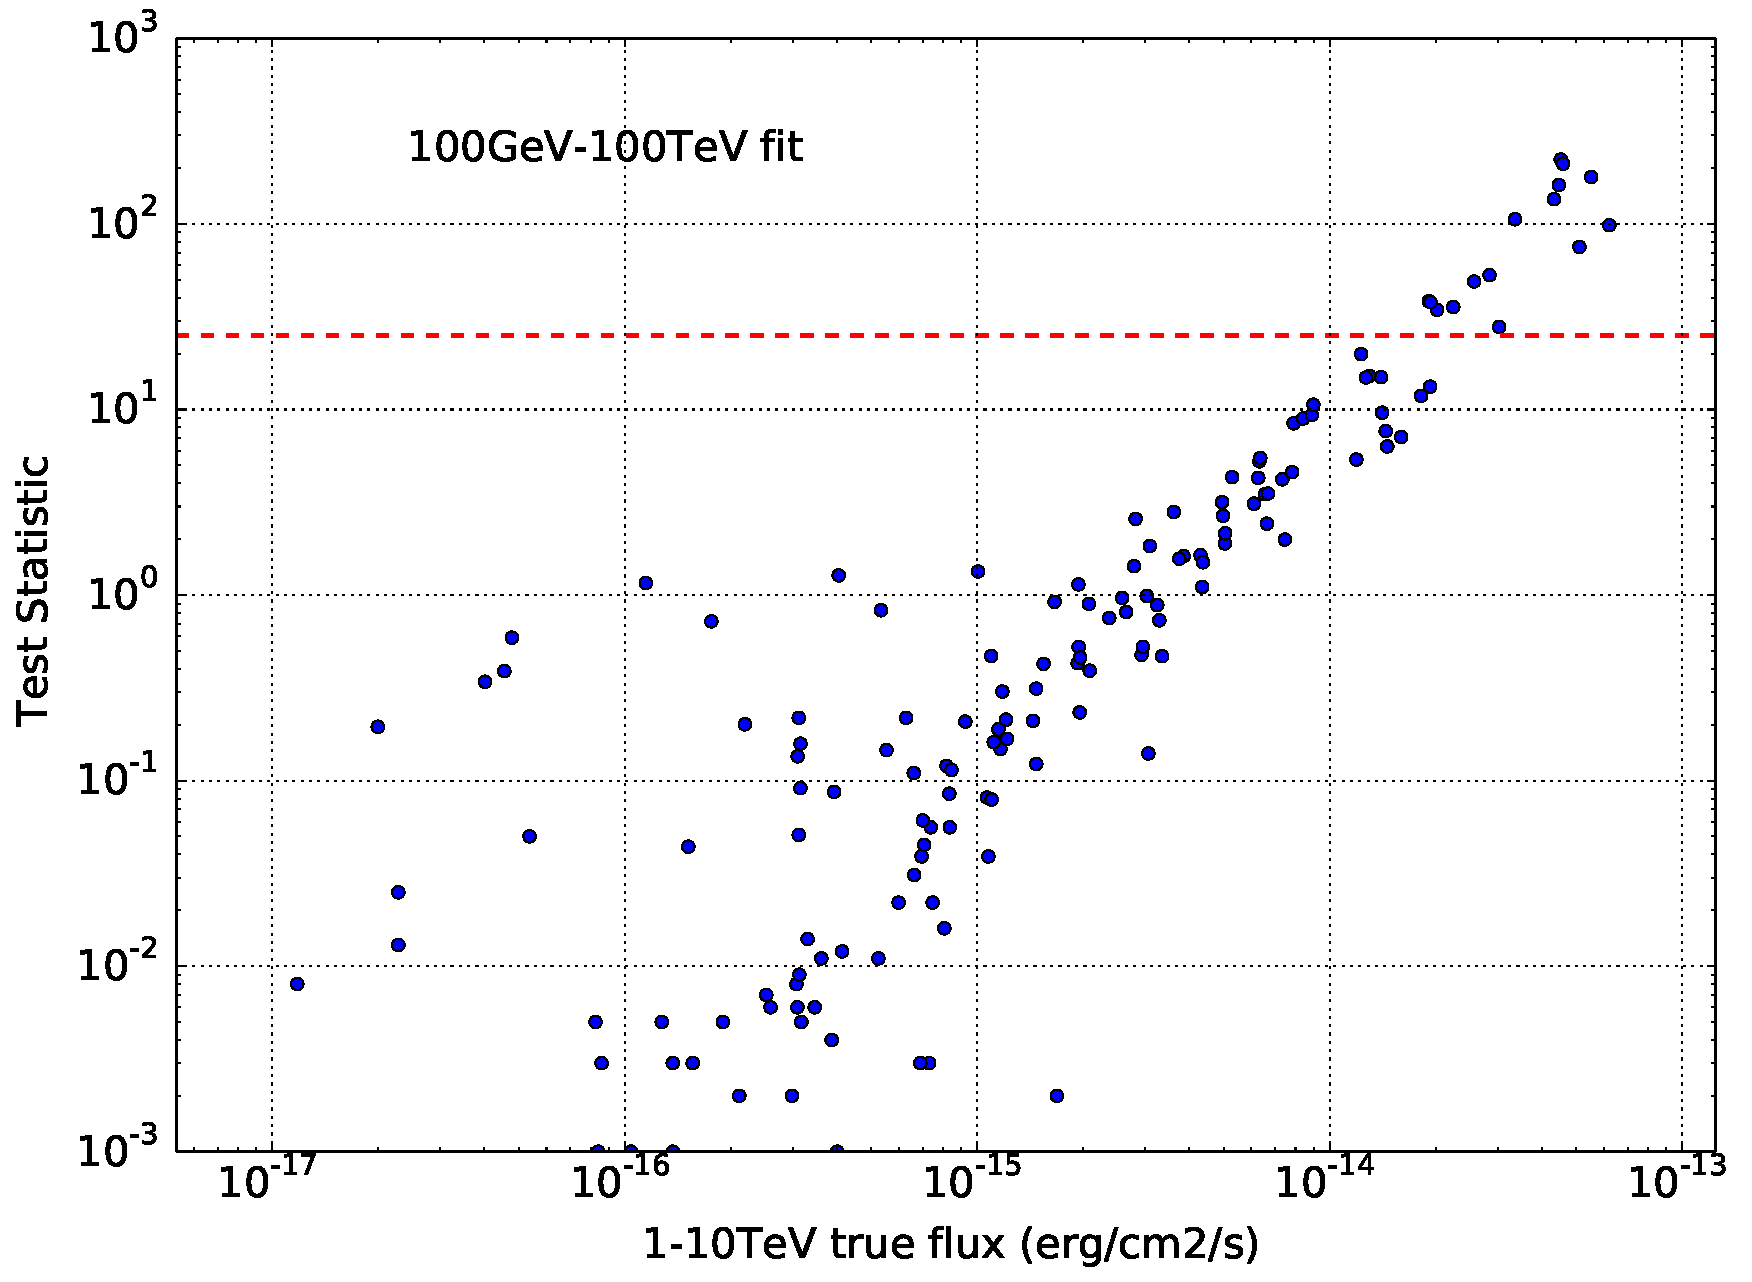
\includegraphics[width=1\textwidth]{Pictures/PWNe-only_TS_100GeV-100TeV_Asimov.pdf}
\endminipage
  \caption{\textit{Left:} True flux vs. fitted flux for the synthetic population of \gls{pwne}. Each \gls{pwn} has been fitted individually, keeping the rest of the model components fixed. \textit{Right:} TS value vs. true flux of the \gls{pwne} population. Red line corresponds to TS=25 ($5\sigma$ detection significance).}
    \label{fig:pwnepopresults}
\end{figure}

\subsection{Diffuse Emission}

The diffuse emission models for pion-decay and \gls{ic} scattering have been fitted as mapcubes where the only free parameter left is the normalization. The fit in the full energy range has resulted in a positive detection for the pion-decay component, with a mean TS value of 29.06 (5.39$\sigma$ significance). A \gls{ts} map for this component has been computed, and is shown in picture \ref{fig:res:pion-tsmap}, where a radial disk with a power law specytrum of 2.5 is used as test source (instead of the true model). The map shows how the regions with higher \gls{ts} values are concentrated in high density gas areas. When modifying the spectrum of the pion-decay model to have a harder spectral index of 2.2 (instead of 2.7 as the baseline model), typical of starburst galaxies, the detection spreads more over the full galaxy.

\begin{figure}[h!]
  \begin{center}
    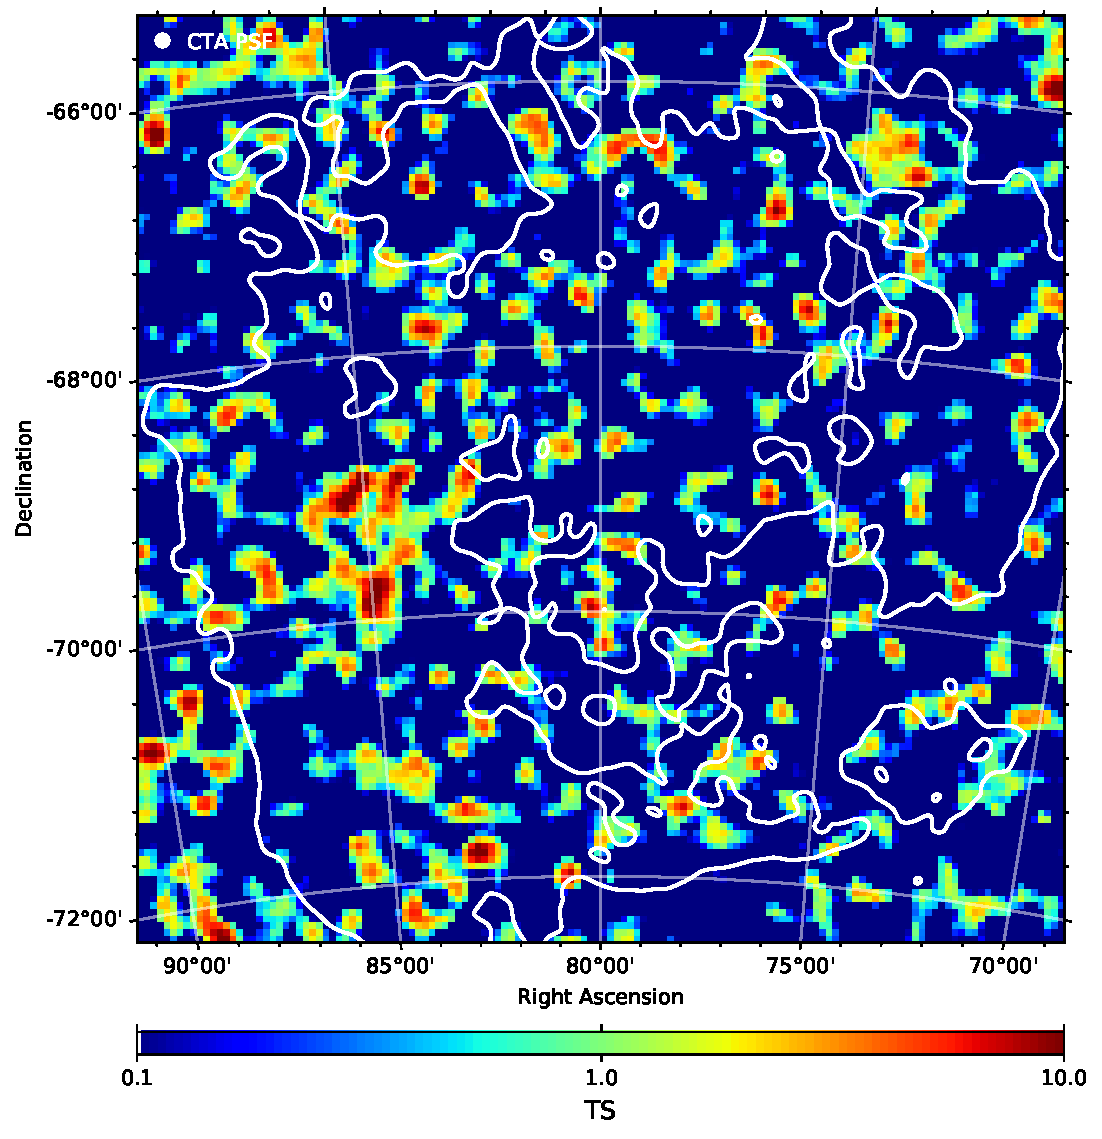
\includegraphics[width=0.45\textwidth]{Pictures/TSmap_Pion_radialdisk010.pdf}
    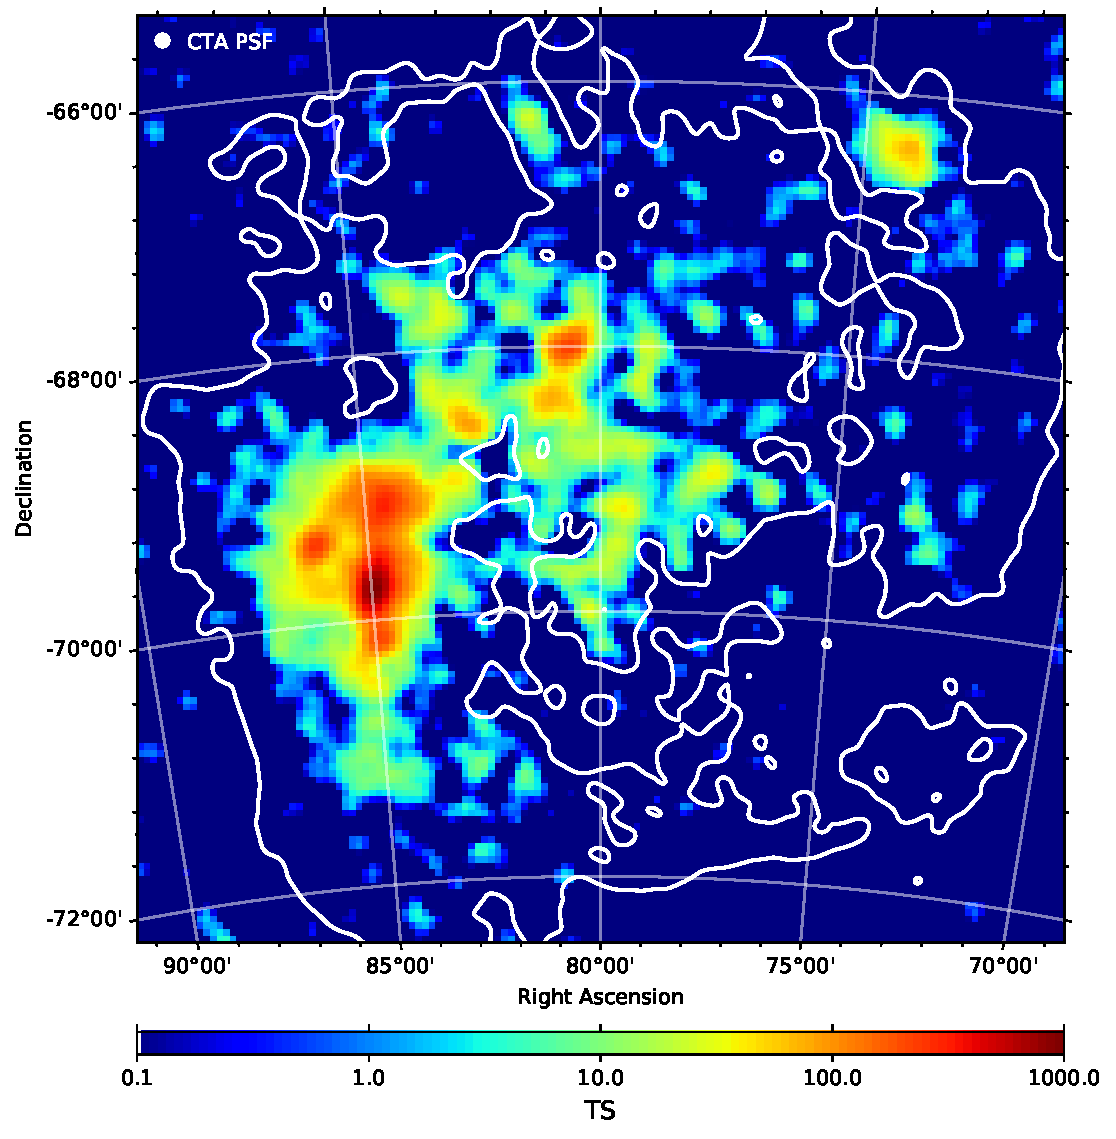
\includegraphics[width=0.45\textwidth]{Pictures/TSmap_Pion-PLidx050_radialdisk010.pdf}
    \caption{\gls{ts} map for simulated observations of the large-scale pion decay emission component computed over 0.1-100 TeV. The test source used to evaluate the \gls{ts} over a grid of positions is a uniform brightness disk of 0.1º radius having a power-law spectrum with fixed photon index 2.5. The left panel shows the \gls{ts} map for the baseline pion decay model, which has photon index of $\sim 2.7$, and the right panel shows the \gls{ts} map obtained for a harder emission model, with photon index of $\sim 2.2$ similar to starburst galaxies.}
    \label{fig:res:pion-tsmap}
  \end{center}
\end{figure}

Regarding the \gls{ic} component, the TS obtained is 0.282, resulting in a non-detection. Upper limits for this model have been calculated instead, giving an upper limit at 99\% confidence level in the integral flux limit of $7.33\cdot10^{-12}$ ph cm$^{-2}$s$^{-1}$ in the range 100 GeV-100TeV. In figure \ref{fig:sensiulimits}, energy flux upper limits for three energy ranges (0.1-1 TeV, 1-10 TeV, 10-100 TeV) are shown.

\begin{figure}[h!]
  \centering
  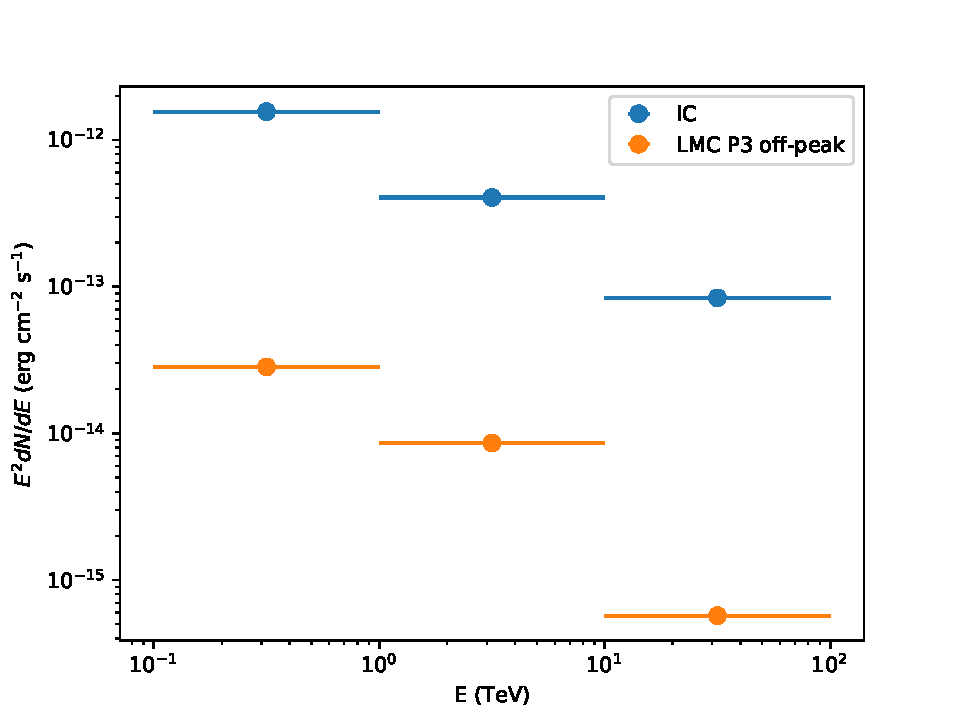
\includegraphics[width=0.7\textwidth]{Pictures/sensicurves_ic+lmcp3.pdf}
  \caption{\label{fig:sensiulimits} Energy flux upper limits computed for the \gls{ic} diffuse component and LMC P3 off-peak model in three energy ranges.}
\end{figure}

\section{Dark Matter annihilation in the LMC} \label{sec:dminlmc}

In this section, an additional component of the diffuse $\gamma$-ray emission in the \gls{lmc}, due to the annihilation of \gls{dm}, is considered. The aim is to find the parameter space of models that could be probed with \gls{cta}, determining if the \gls{lmc} is a good candidate to set contraints on the \gls{wimp} \gls{dm} model.\\
The assumption is that \gls{dm} is composed by stable particles which can annihilate and produce a shower of \gls{sm} particles, which in turn would lead to either direct or secondary production of $\gamma$-rays, as explained in section \ref{sec:DM}. The range of energies for this process can go from a few GeV to several TeV, making it potentially observable by \gls{cta}. It must be taken into account that there exists plenty of \gls{dm} candidates in the literature \cite{2004DMcandidates}, \cite{2005DMcandidates}, \cite{2009DMcandidates}, but in this work only the \glspl{wimp} annihilation scenario is considered.\\
The flux of $\gamma$-rays produced by \gls{dm} annihilation was presented in equation \ref{eq:flux}, reproduced here for convenience:

\begin{equation}
    \frac{d \Phi}{dE}=\frac{1}{8 \pi} \frac{<\sigma v>}{m_{\chi}^2} \frac{d N_{\gamma}}{dE} \int_{\Delta\Omega}\int_{l.o.s} dl \rho^2(\vec{l})
\label{eq:flux-dm}
\end{equation}

Where $dN/dE$ is the spectrum of $\gamma$-rays from annihilation of a pair of dark matter particles, $\langle\sigma v\rangle$ is the thermal velocity averaged annihilation cross section, $m_\chi$ is the \gls{dm} particle mass and $\rho$ is the dark matter density profile. If \gls{dm} particle is not its own antiparticle, equation \ref{eq:flux-dm} should be multiplied by a factor 1/2. \\
Along the full analysis, the mass of the \gls{dm} particle and the annihilation cross section will be cosnidered free parameters, fixing the rest of the model features. A single annihilation spectra will be assumed where the branching ratio of the reaction is one, meaning that the entire annihilation happens in a specific channel. The results will be presented in the shape of sensitivity curves where the minimum annihilation cross section needed for detection is plotted against the mass of the \gls{dm} particle for a specific annihilation channel and \gls{dm} profile.

\subsection{Dark Matter profile in the \gls{lmc}}

The \gls{dm} distribution of the \gls{lmc} can be inferred by the gravitational structure of its disk, following the rotation curve method. Assuming circular orbits, the mass of a galaxy enclosed in a certain radius can be calculated thanks to the rotation velocity, $v_{rot}$ = GM(<r)/r. Measurements of the rotation velocities of stars and gas in the \gls{lmc} allow to calculate the total mass \cite{LMCHI}, and subtracting the contribution to the rotation curve of the luminous matter, the remaining \gls{dm} mass can be estimated. The dark matter profiles used in this section rely on the works of \cite{2015FermiLMCDM}, where the gas mass component of HI+He as a function of the radius is taken from \cite{1992gasLMC}; and the stellar mass is extracted from \cite{2006LMCkinematics}. The rotation curve of the \gls{lmc} can be seen in picture \ref{fig:rotcurve}.\\
A generalized six-parameter Hernquist-Zhao \gls{dm} profile has been adopted for this work (\cite{1990Hernquist}, \cite{1996Zhao}), following equation \ref{eq:gnfw} from section \ref{sec:DM}, reproduced here for convenience:


\begin{equation}
    \rho(r) = \frac{2^{\frac{\beta-\gamma}{\alpha}} \times \rho_{0}}{\left(\frac{r}{r_{S}}\right)^{\gamma}\left[ 1+\left(\frac{r}{r_{S}} \right)^{\alpha}\right]^{\frac{\beta-\gamma}{\alpha}}}\Theta(r_{max}-r)
\end{equation} \label{fig:gnfw}

Where $\Theta$ is the Heaviside step function, $r_{S}$ is the scale radius and $\rho_{0}$ is the characteristic density. These two last parameters are properties of the specific \gls{dm} halo. Setting $(\alpha,\beta,\gamma) = (1,3,1)$ we retrieve the \gls{nfw} profile \cite{NFW} \footnote{When $\alpha$ = 1 and $\beta$ = 3 the Zhao profile is typically called generalised NFW profile (gNFW) with flexible inner \gls{dm} density slope $\gamma$.}. An isothermal profile is obtained setting $(\alpha,\beta,\gamma) = (2,2,0)$. Variations of these two profiles have been tested, with their parameters shown in table \ref{tab:dmprofiles} and plotted in figure \ref{fig:dmprofiles}. For the \gls{nfw} profile, a more cuspy profile with $\gamma=1.5$ and a more cored profile, with $\gamma=0.5$ are tested. In the case of the isothermal profile, the scale radius is varied from the iso-mean profile with $r_{S}$ = 2.4 (kpc) to iso-max with $r_{S}$ = 3 (kpc) and iso-min with $r_{S}$ = 1 (kpc).

\begin{figure}[h!]
  \centering
  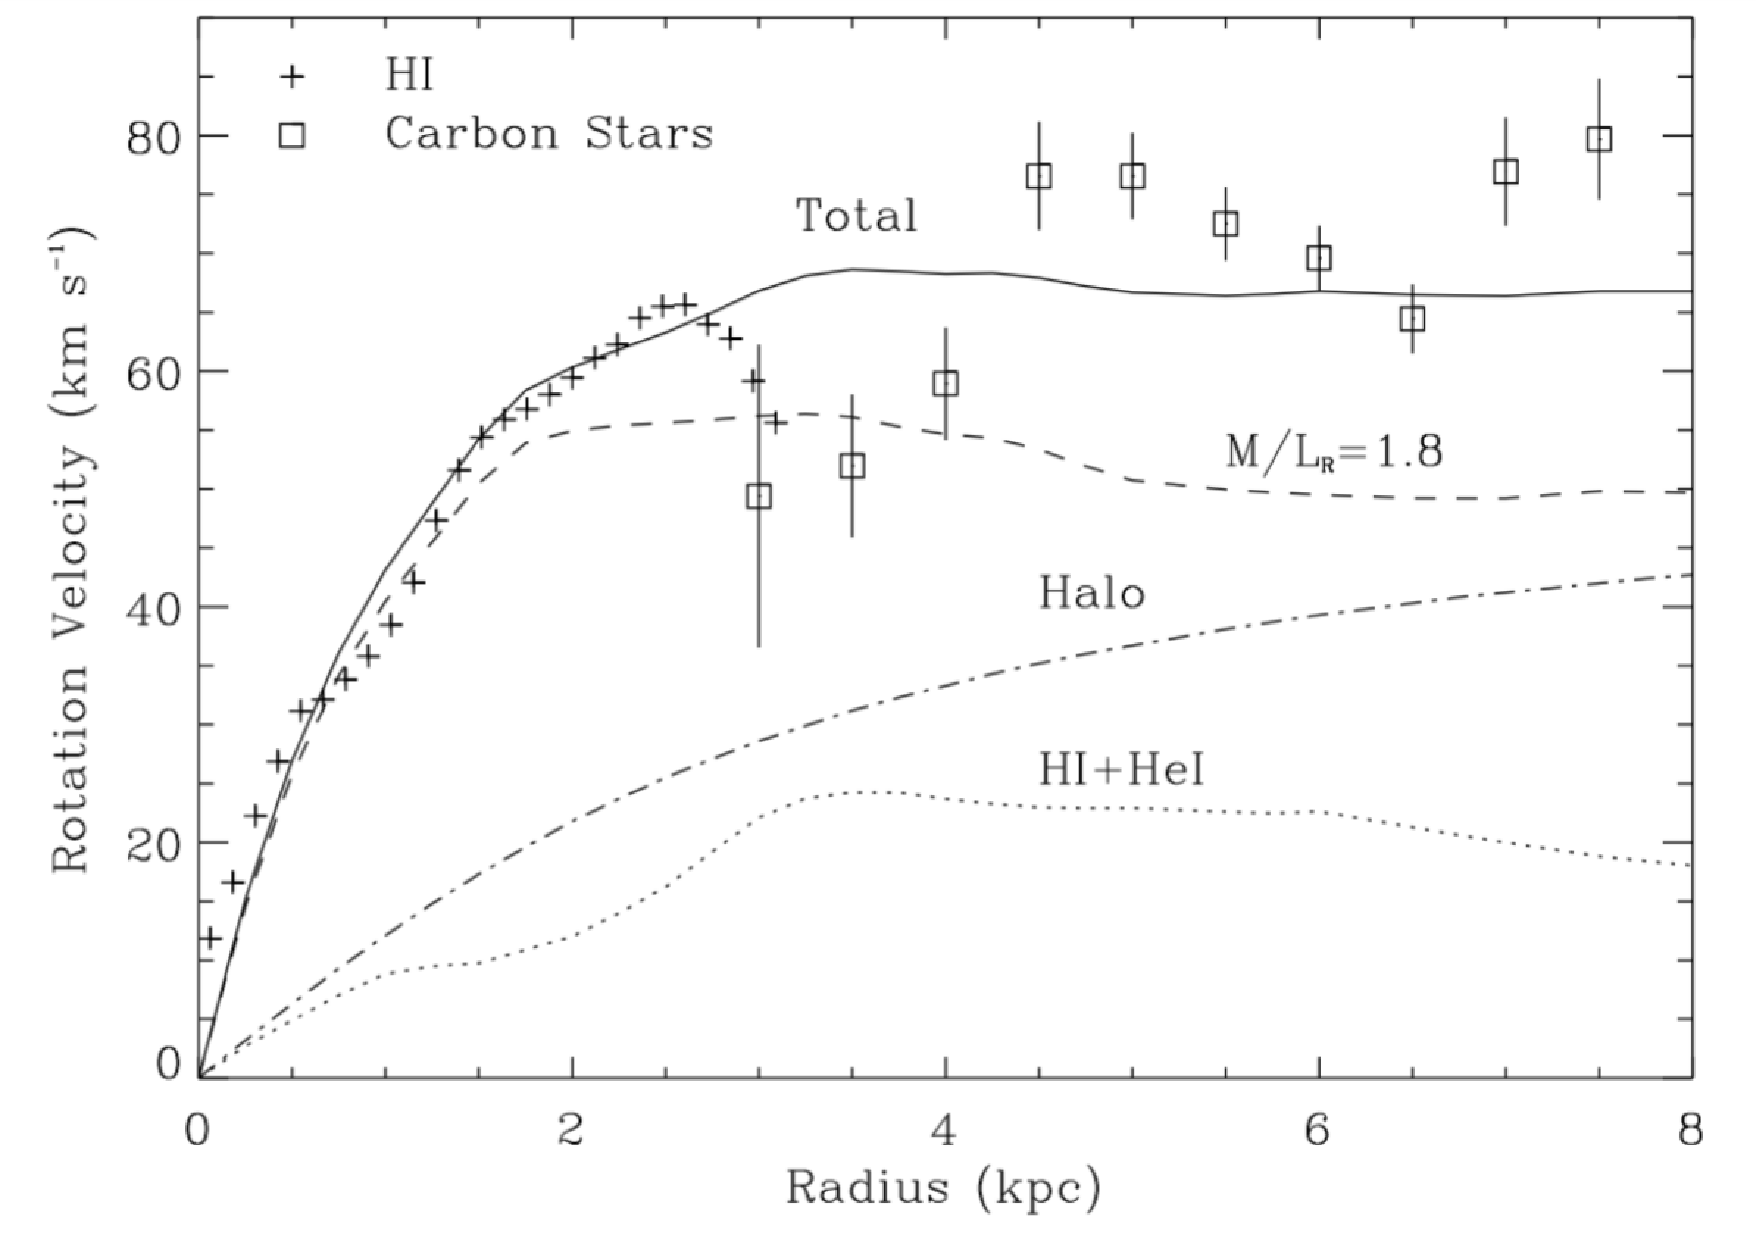
\includegraphics[width=0.7\textwidth]{Pictures/rotationcurvelmc.pdf}
  \caption{\label{fig:rotcurve} Rotation curve of the \gls{lmc}, from \cite{LMCHI}. The solid black line is the total predicted rotation curve constructed from the following components: (\textit{a}) HI mass distribution from \cite{1992gasLMC}, and a 30\% He contribution (\textit{dotted line}). (\textit{b}) R stellar light distribution based on the data from \cite{1958starsinLMC} and $M/L_{R}=1.8$ (dashed line). (\textit{c}) Pseudoisothermal dark halo with core radius 2.5 kpc and central densiy $0.009 M_{\odot}$pc$^{-3}$.}
\end{figure}

\begin{figure}[h!]
  \centering
  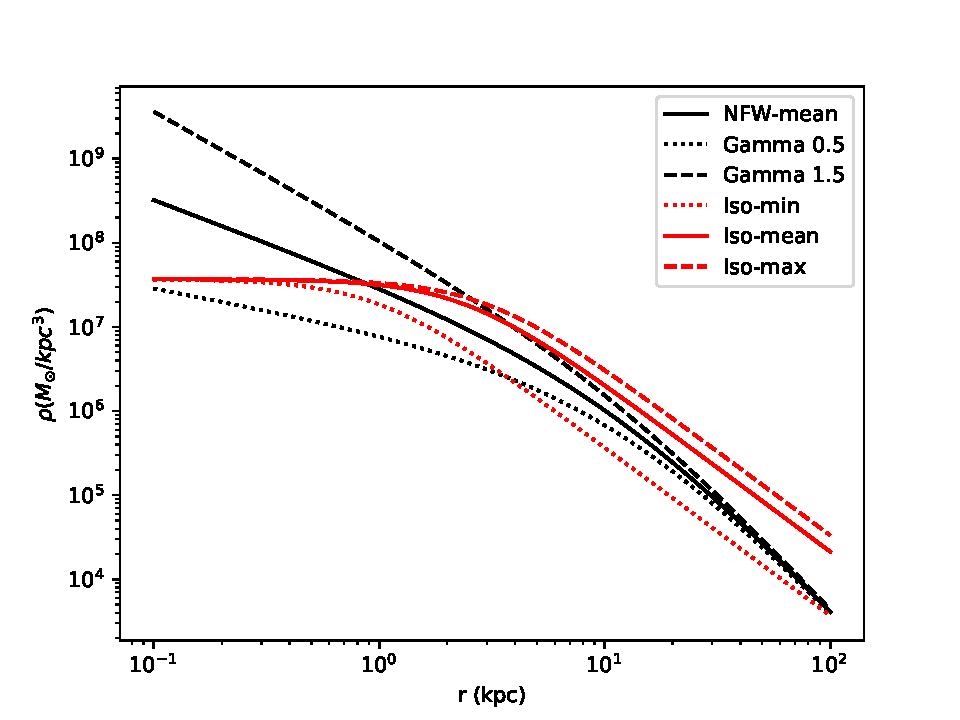
\includegraphics[width=0.7\textwidth]{Pictures/dmprofiles.pdf}
  \caption{\gls{dm} profiles plotted against the radius $r$ from the \gls{lmc} center, with the parameters listed in table \ref{tab:dmprofiles}.} \label{fig:dmprofiles}
\end{figure}

\begin{table}
  \centering
  \resizebox{\textwidth}{!}{%
    \begin{tabular}{lllllll}
      \hline
      Profile & $\alpha$ & $\beta$ & $\gamma$ & $r_{S} (kpc)$ & $\rho_{0} (M_{\odot}/kpc^3)$ & $J(10º) (GeV^{2}/cm^5)$\\
      \hline
      NFW-mean & 1 & 3 & 1 & 12.6 & $2.6\times10^6$ & $1.36 \times 10^{21}$ \\
      NFW-core & 1 & 3 & 0.5 & 12.6 & $2.6\times10^6$ & $5.13 \times 10^{20}$ \\
      NFW-cuspy & 1 & 3 & 1.5 & 12.6 & $2.6\times10^6$ & $4.22 \times 10^{22}$\\
      Iso-min & 2 & 2 & 0 & 1 & $3.7\times10^7$ & $8.51\times 10^{19}$ \\
      Iso-mean & 2 & 2 & 0 & 2.4 & $3.7\times10^7$ & $9.71\times 10^{20}$\\
      Iso-max & 2 & 2 & 0 & 3 & $3.7\times10^7$ & $1.74\times 10^{21}$ \\
      \hline
    \end{tabular}}
    \caption{Parameters of the \gls{dm} profiles used in this work. Values of NFW-mean and Iso-mean profiles are the same as of \cite{2015FermiLMCDM}. The $J$-factors are integrated over 10º from the halo center.} \label{tab:dmprofiles}
\end{table}

The \gls{dm} profiles were simulated using the software \textit{clumpy}, a code for $\gamma$-ray and neutrino signals from \gls{dm} structures \cite{2019CLUMPY}. It allows to compute simulations of \gls{dm} halos characterized by a series of parameters depending on the \gls{dm} profile. \textit{Clumpy} was used in this work to simulate maps of the J-factor in the region of the \gls{lmc} in order to create the spatial distribution of the different \gls{dm} models, which afterwards were combined with the spectrum of several annihilation channels to reproduce the $\gamma$-ray flux in the \gls{lmc}. The 2D J-factor of the different profiles used in this work, computed with \textit{clumpy} can be seen in figure \ref{fig:jfactors}.

\begin{figure}[h]
\centering
\minipage{0.5\textwidth}
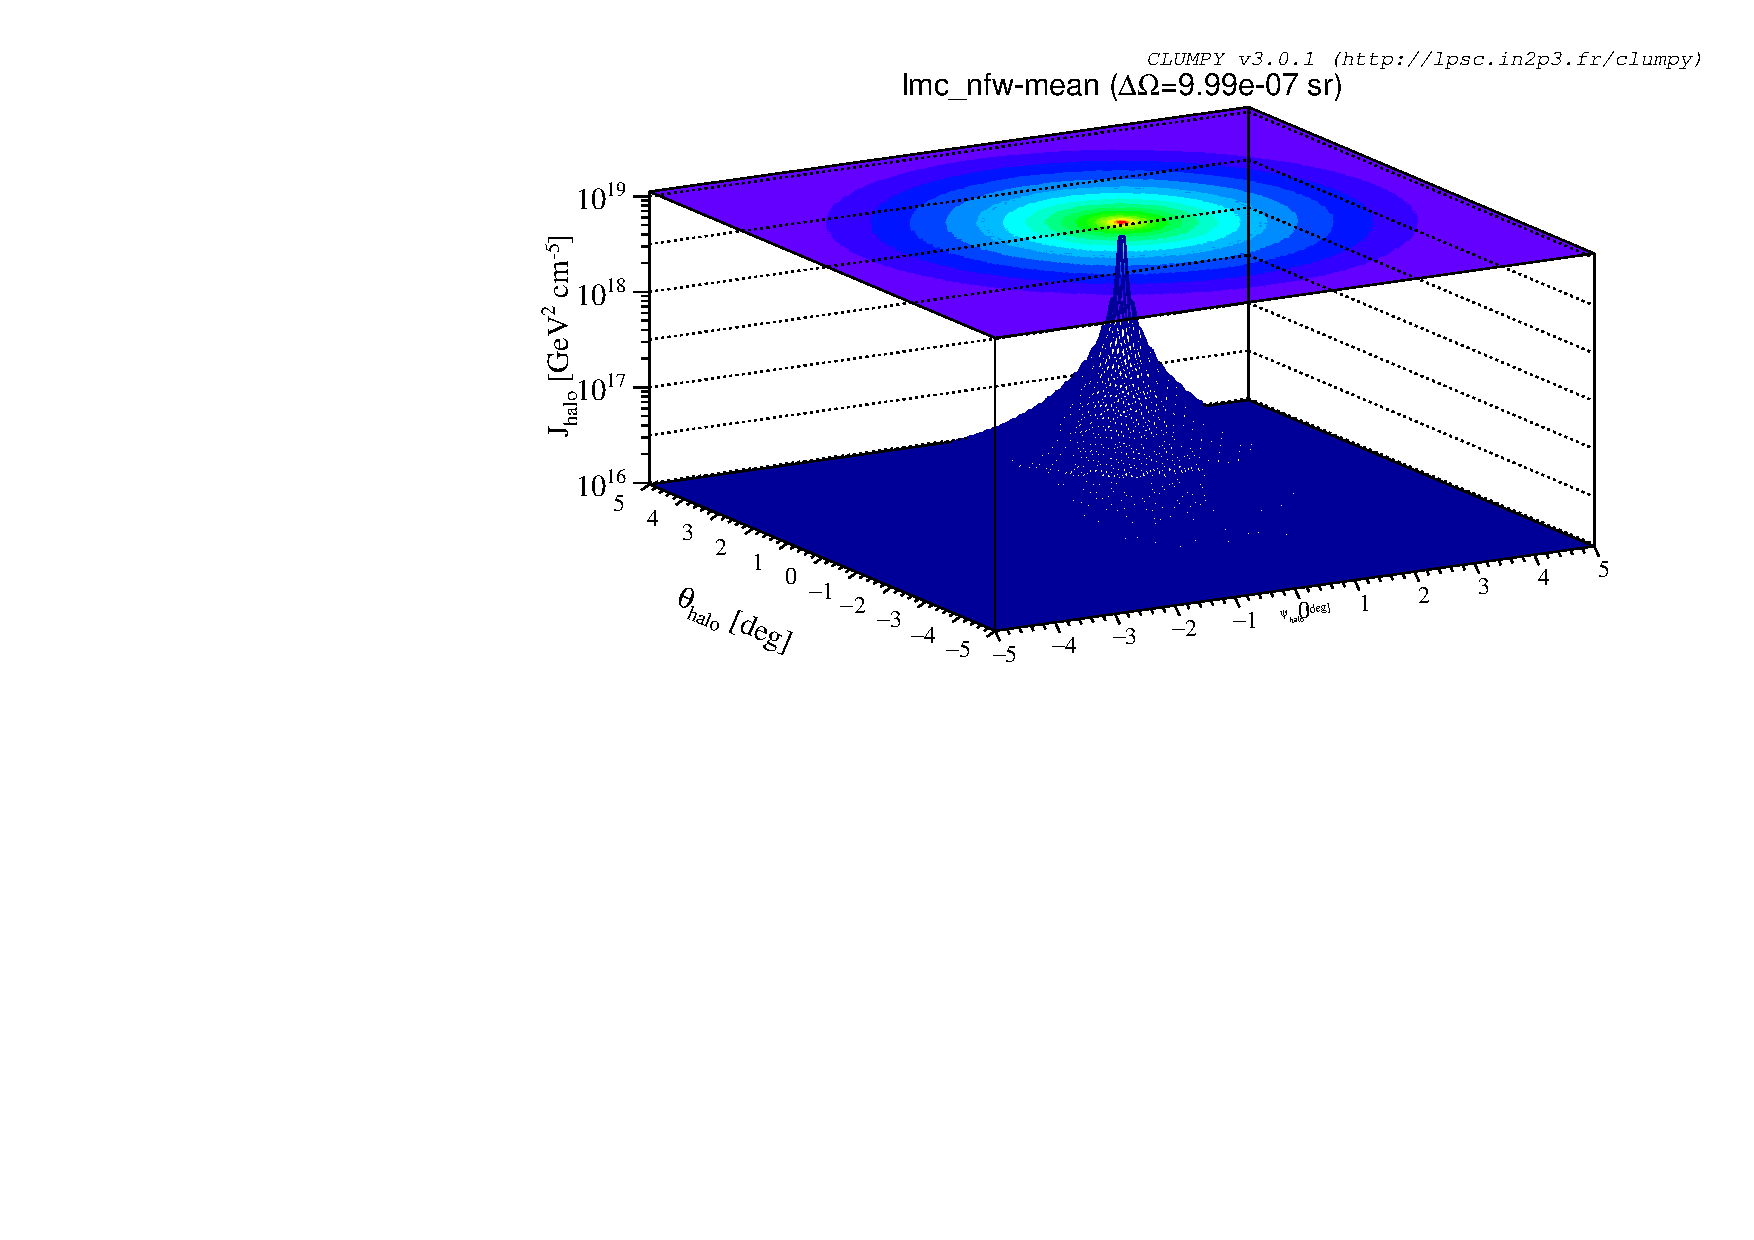
\includegraphics[width=1\textwidth]{Pictures/lmc_nfw-mean.pdf}
\endminipage 
\minipage{0.5\textwidth}
\includegraphics[width=1\textwidth]{Pictures/lmc_iso-mean.pdf}
\endminipage \\
\minipage{0.5\textwidth}
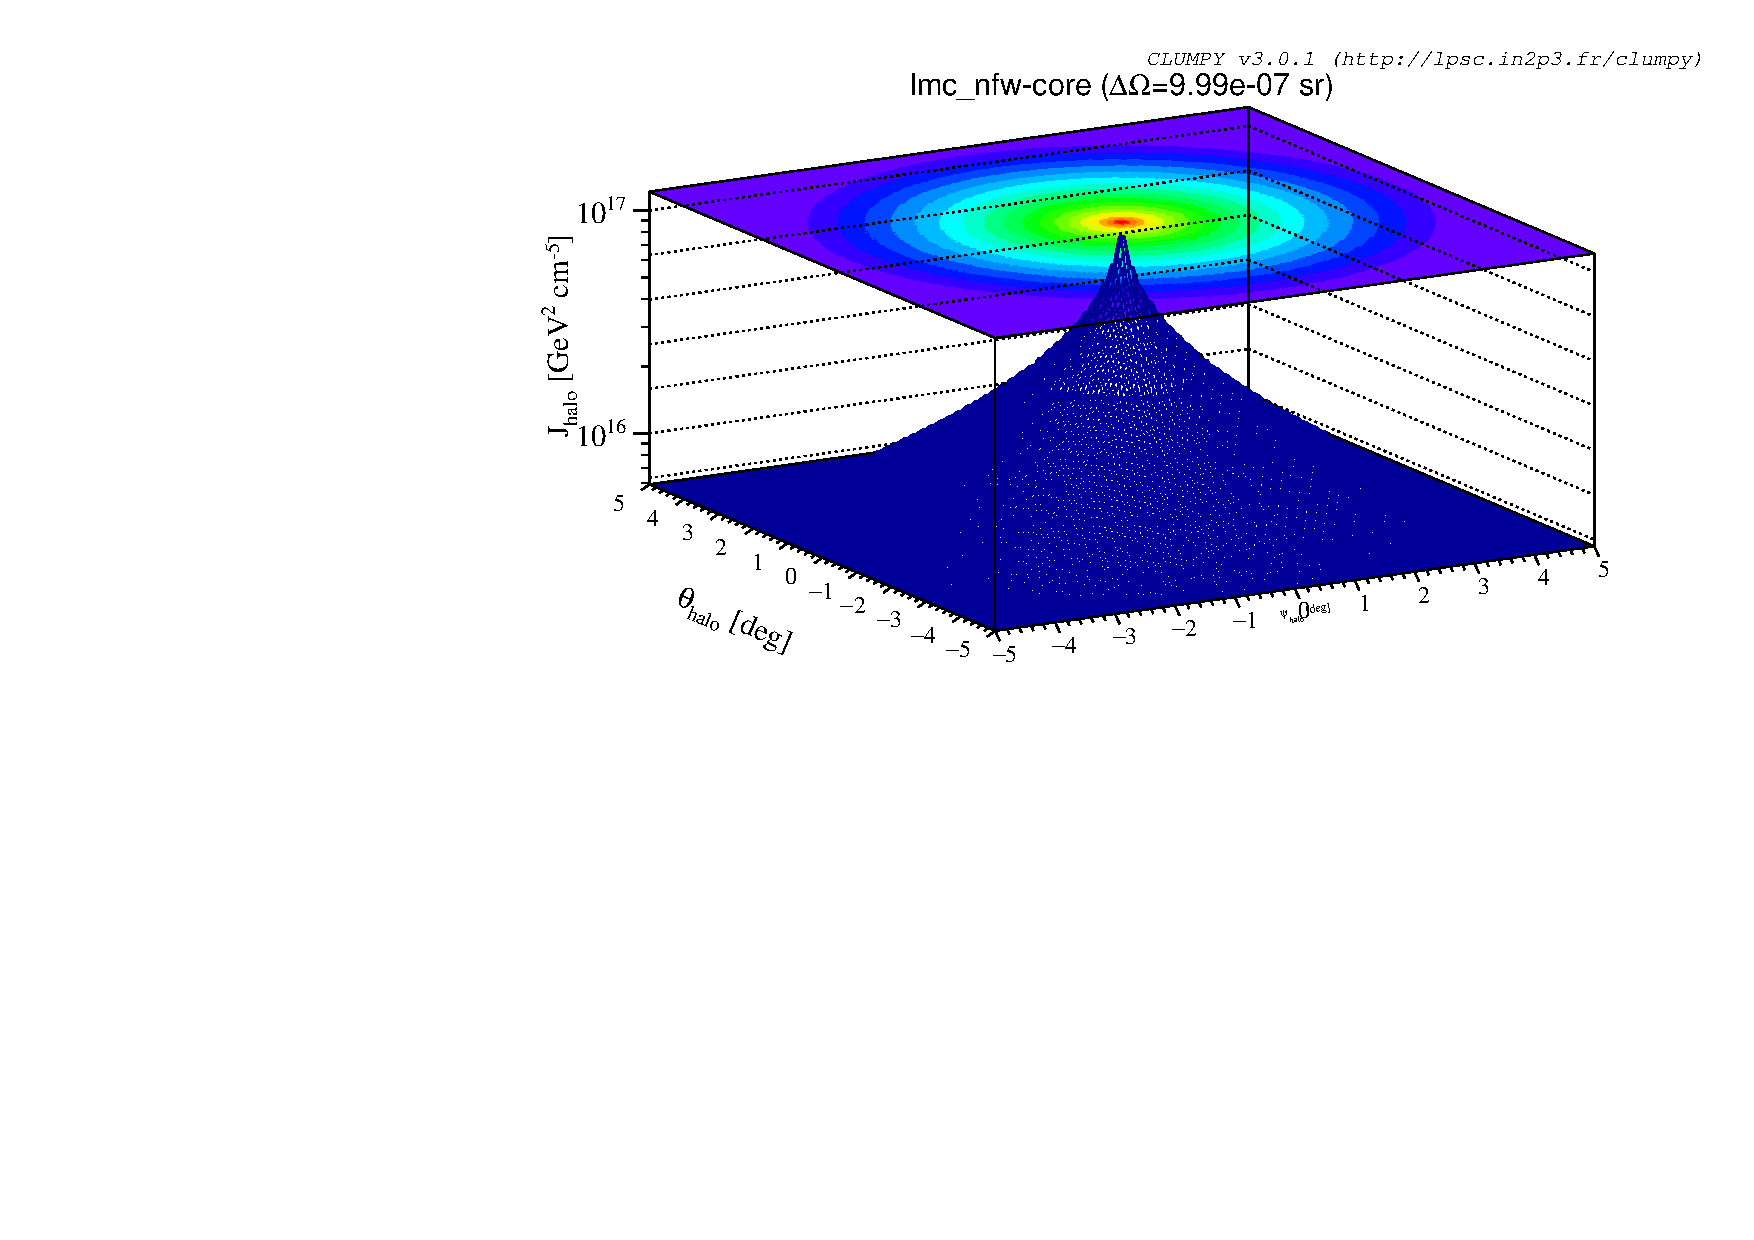
\includegraphics[width=1\textwidth]{Pictures/lmc_nfw-core.pdf}
\endminipage
\minipage{0.5\textwidth}
\includegraphics[width=1\textwidth]{Pictures/lmc_iso-min.pdf}
\endminipage \\
\minipage{0.5\textwidth}
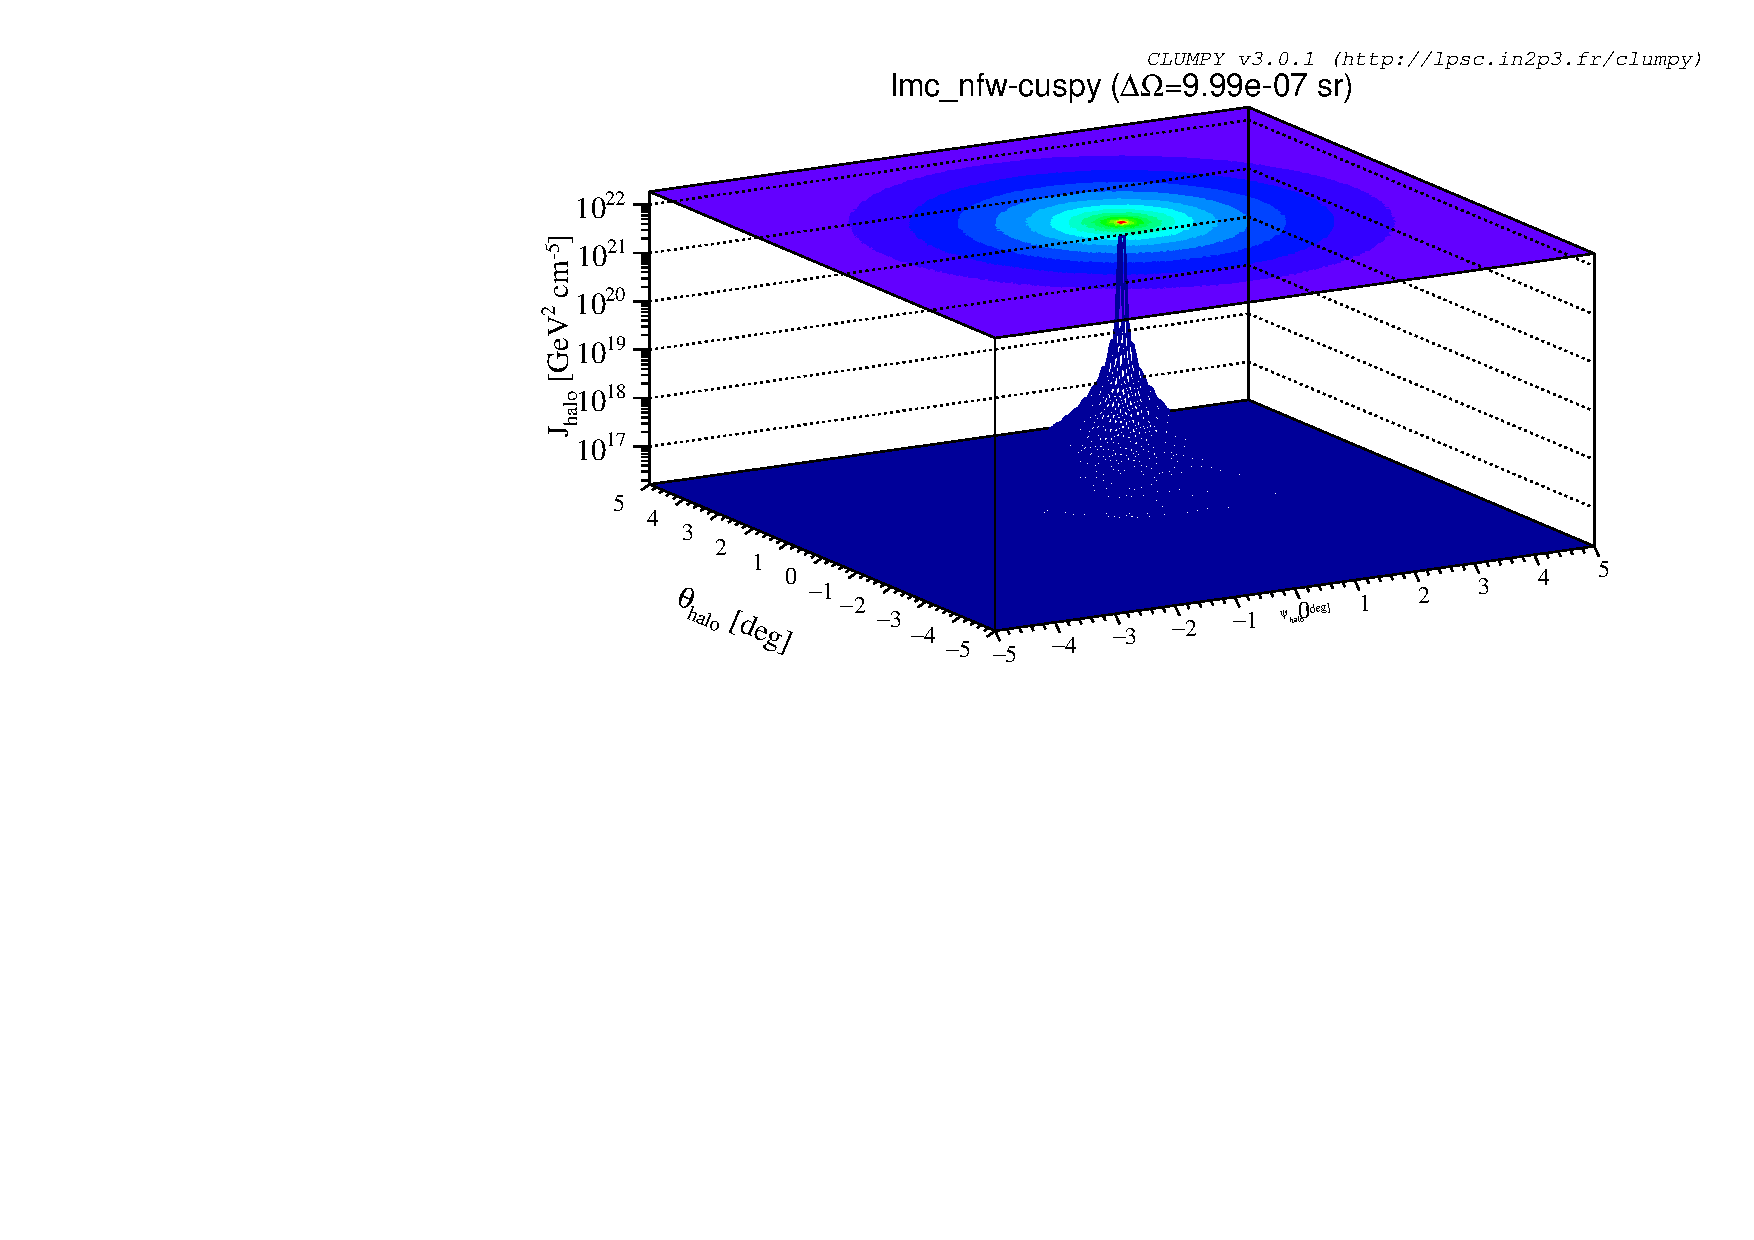
\includegraphics[width=1\textwidth]{Pictures/lmc_nfw-cuspy.pdf}
\endminipage
\minipage{0.5\textwidth}
\includegraphics[width=1\textwidth]{Pictures/lmc_iso-max.pdf}
\endminipage
  \caption{2-D J-Factors of the \gls{lmc} \gls{dm} profiles probed in this work. The \gls{nfw} and Isothermal profiles were computed using the same parameters as in \cite{2015FermiLMCDM}.}
    \label{fig:jfactors}
\end{figure}

\subsection{$\gamma$-ray spectrum}

For the spectral part of the \gls{dm} emission model ($dN_{\gamma}/dE$ in equation \ref{eq:flux}), the methodology from \cite{2011cirelli} was followed, where the energy spectra of $\gamma$-rays produced by different \gls{dm} annihilation channels are provided. For this thesis, the studied channels were $b \overline b$, $W^+ W^-$, $\tau^+\tau^-$, $\mu^+ \mu^-$ including electro-weak corrections as computed in \cite{2011EWcorrections}. The annihilation spectral flux of these channels is shown in figure \ref{fig:dmspec}, computed for a set of \gls{dm} particle masses.

\begin{figure}[h!]
  \centering
  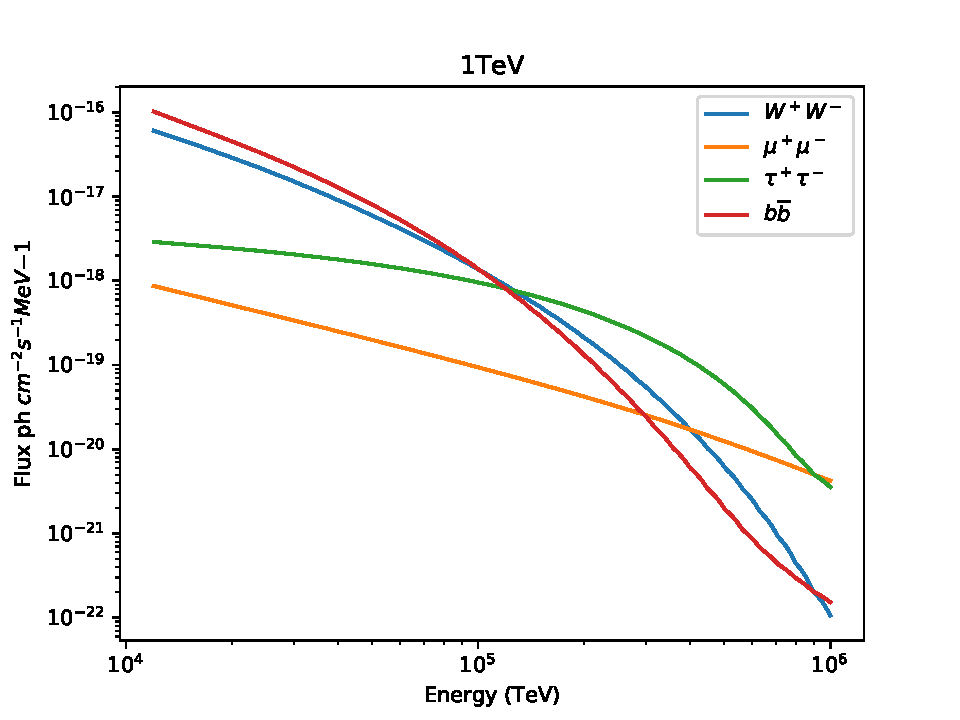
\includegraphics[width=0.5\textwidth]{Pictures/1tevspectra.pdf}
  \minipage{0.4\textwidth}
  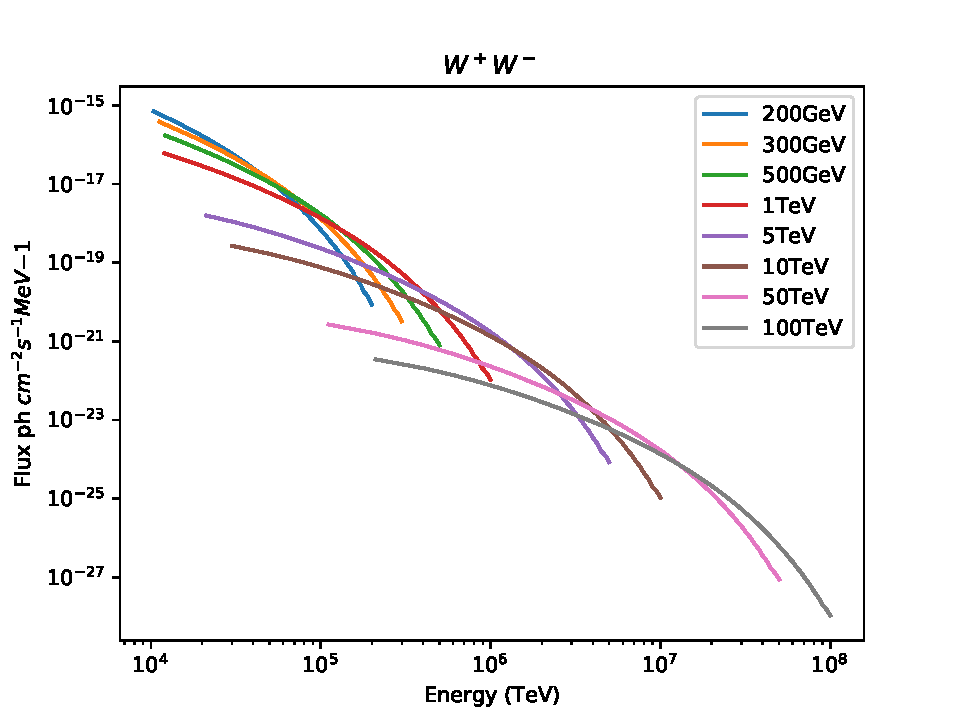
\includegraphics[width=1\textwidth]{Pictures/specW.pdf}
  \endminipage 
  \minipage{0.4\textwidth}
  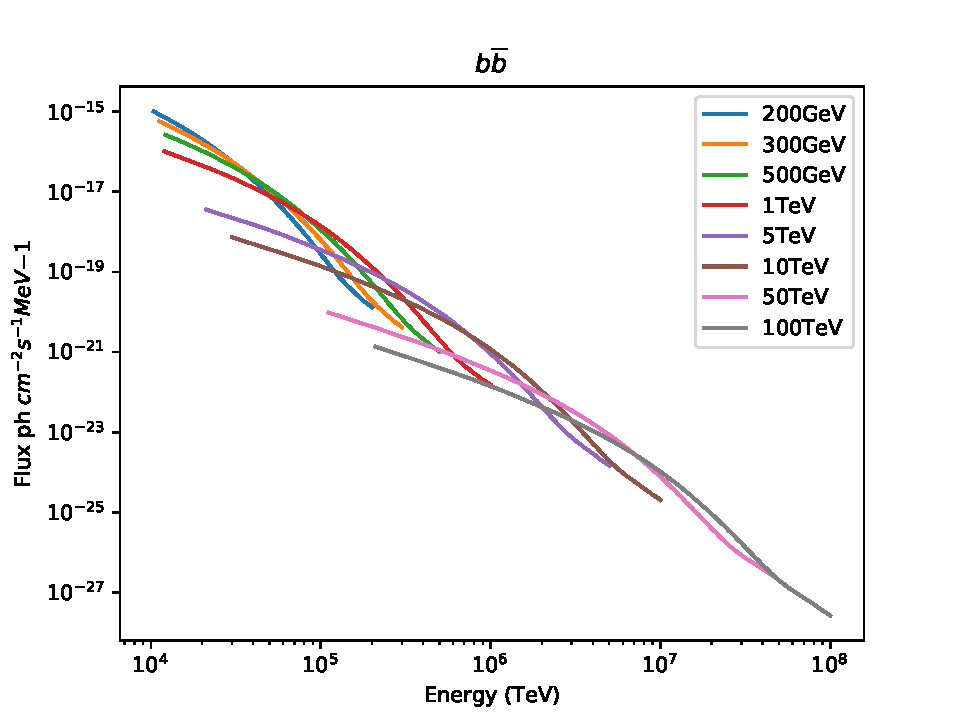
\includegraphics[width=1\textwidth]{Pictures/specb.pdf}
  \endminipage \\
  \minipage{0.4\textwidth}
  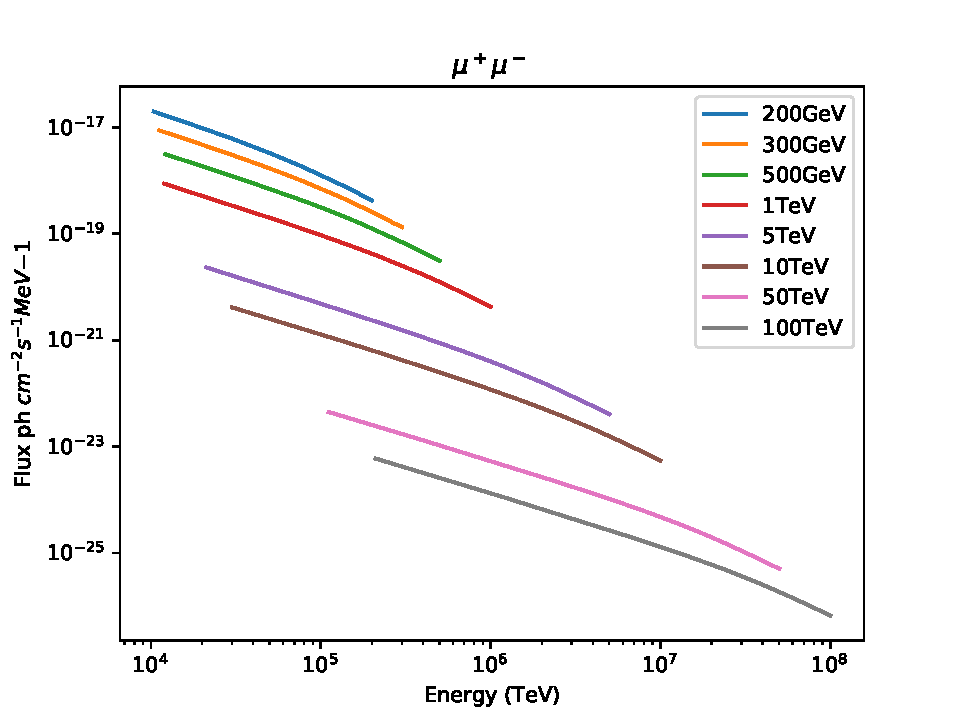
\includegraphics[width=1\textwidth]{Pictures/specMu.pdf}
  \endminipage
  \minipage{0.4\textwidth}
  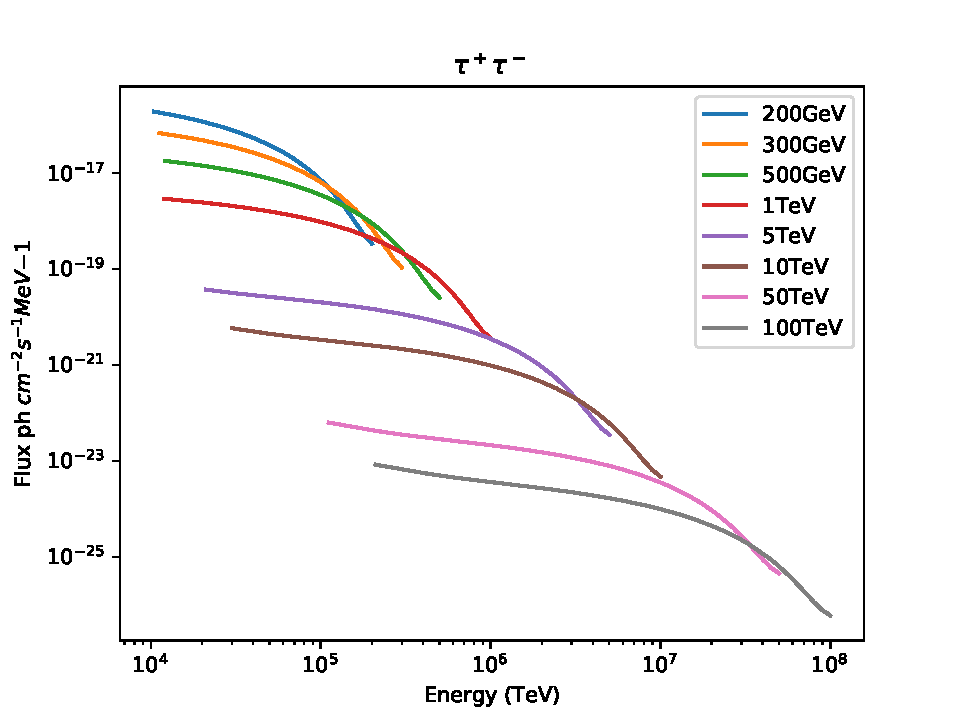
\includegraphics[width=1\textwidth]{Pictures/specTau.pdf}
  \endminipage \\
  \caption{Flux of $\gamma$-rays produced by \gls{dm} pair annihilation, for different annihilation channels and masses of the \gls{dm} particle. }
  \label{fig:dmspec}
\end{figure}

\subsection{Results on \gls{dm} sensitivity curves}

Using the \gls{dm} profiles and spectra described in previous sections, a likelihood analysis was performed to obtain the minimum flux needed for the \gls{lmc} \gls{dm} component to be detectable by \gls{cta}. The Asimov data set with the astrophysical $\gamma$-ray sources described in section \ref{sec:model} is used for this task as a background on top of which the flux needed to be emitted by each \gls{dm} model in order to be detected is calculated. To do so, the procedure for upper limits calculation described in section \ref{sec:ulimits} is applied. Each \gls{dm} model is included in the model as a new test source, for which the differential upper flux limit for a reference energy, the integrated upper flux limit over the energy range from 0.1 GeV to the \gls{dm} particle mass, and the integrated energy limit are calculated.\\
From the resulting flux $\frac{d \Phi_{ulim}}{dE}$, replacing the value in equation \ref{eq:flux-dm}, the limit on the velocity averaged annihilation cross section $<\sigma v>$ can be extracted. The sensitivity curves where $<\sigma v>$ is plotted versus \gls{dm} particle masses are shown in picture \ref{fig:dmsensicurves}. Each curve corresponds to a specific \gls{dm} profile and annihilation channel. The space above the curves represent the parameter space of $<\sigma v>$ and \gls{dm} mass that could be detected by \gls{cta}. Since the results on the Asimov dataset only provide mean values, it must be taken into account that these sensitivity curves are subject to uncertainties due to poissonian fluctuations of the data, and systemathics. However, because the curves are several orders of magnitude above the canonical thermal cross section (which is the one supported by \gls{wimp} theory), it has not been considered necessary to perform a detailed analysis of these uncertainties, which would unlikely reach the region of the canonical thermal cross section anyway.

\begin{figure}[h!]
\centering
\minipage{0.5\textwidth}
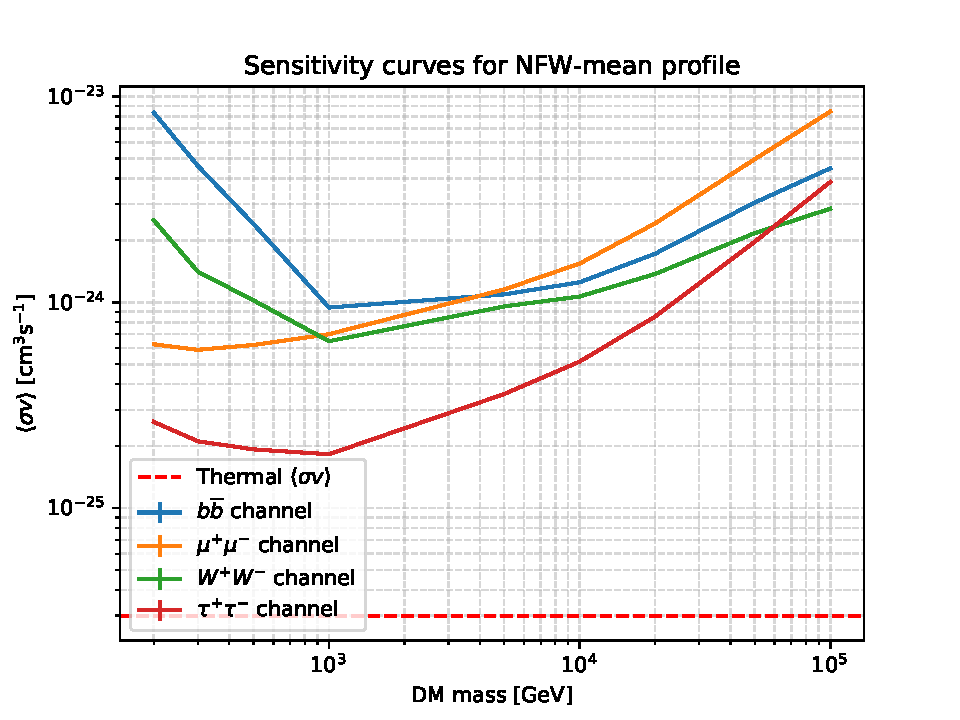
\includegraphics[width=1\textwidth]{Pictures/Limits_NFW-mean.pdf}
\endminipage 
\minipage{0.5\textwidth}
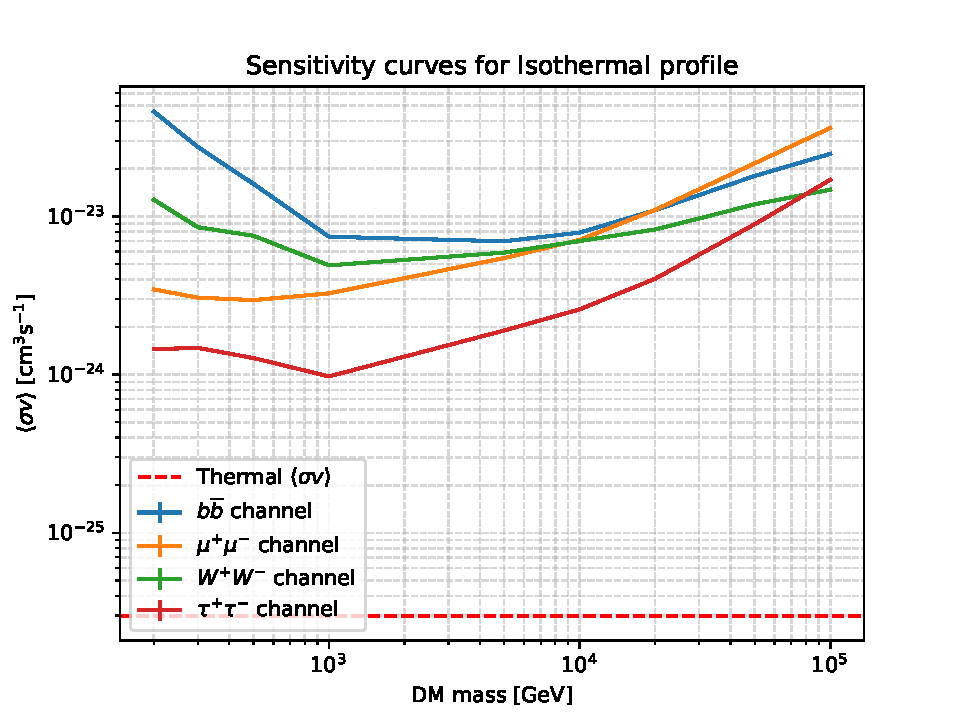
\includegraphics[width=1\textwidth]{Pictures/Limits_Isothermal.pdf}
\endminipage \\
\minipage{0.5\textwidth}
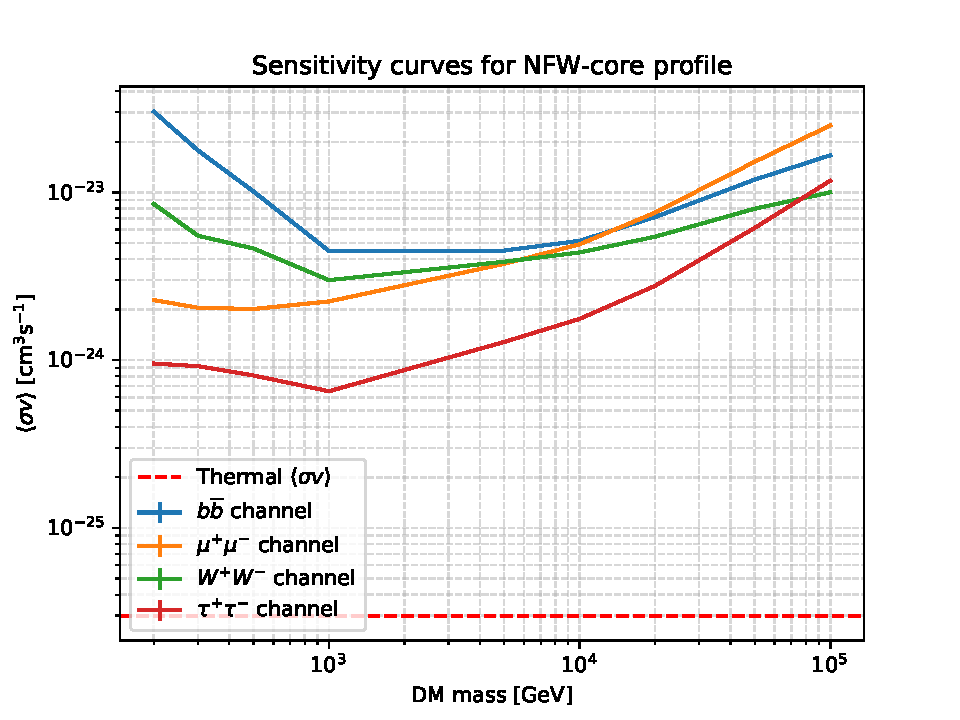
\includegraphics[width=1\textwidth]{Pictures/Limits_NFW-core.pdf}
\endminipage
\minipage{0.5\textwidth}
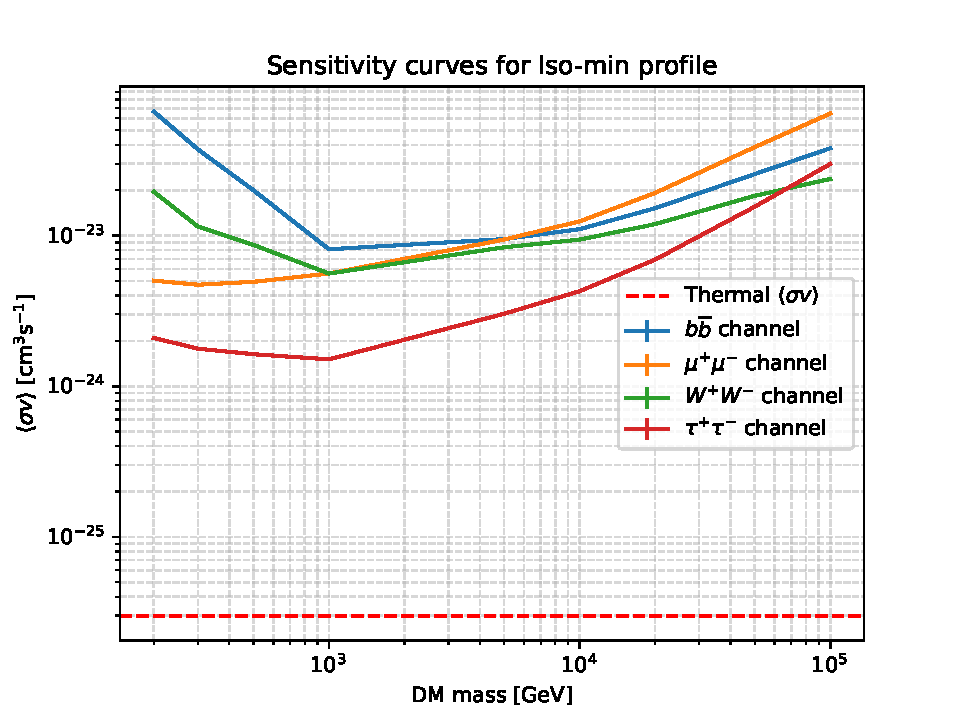
\includegraphics[width=1\textwidth]{Pictures/Limits_Iso-min.pdf}
\endminipage \\
\minipage{0.5\textwidth}
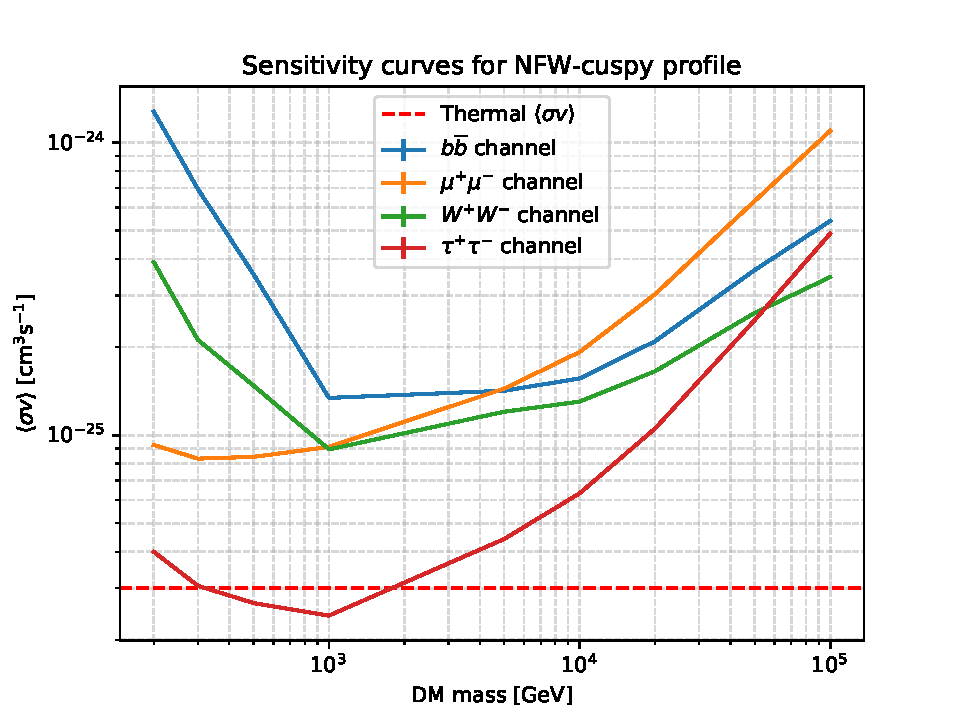
\includegraphics[width=1\textwidth]{Pictures/Limits_NFW-cuspy.pdf}
\endminipage
\minipage{0.5\textwidth}
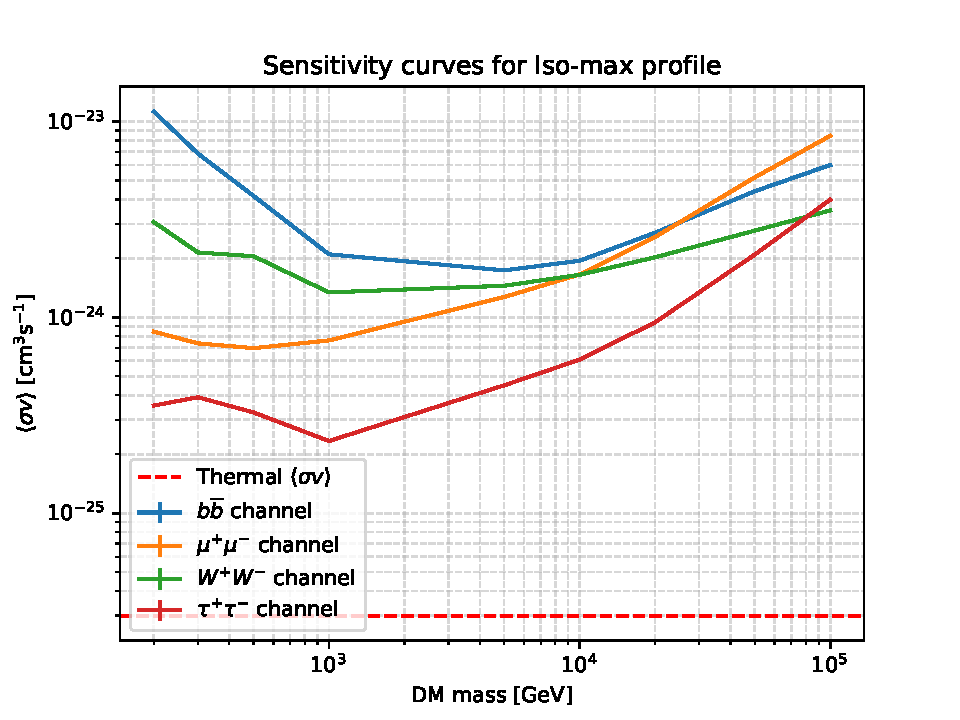
\includegraphics[width=1\textwidth]{Pictures/Limits_Iso-max.pdf}
\endminipage
  \caption{Sensitivity curves of $<\sigma v >$ vs. \gls{dm} particle mass, resulting for the profiles listed in table \ref{tab:dmprofiles}, and for four annihilation channels: $b\overline b$, $W^+W^-$, $\mu^+ \mu^-$, $\tau^+ \tau^-$.}
    \label{fig:dmsensicurves}
\end{figure}

\subsection{Effect of the diffuse emission on the DM sensitivity curves}  \label{sec:dm:diff}

Since the \gls{lmc} is observed as an extended object and present a particular structure in its diffuse $\gamma$-ray emission, it offers the unique opportunity to study the influence of this extended emission in the detection of \gls{dm}. The differences in the spatial structure of the diffuse $\gamma$-ray emission,  which is correlated with \gls{cr} accelerartion sources, and the \gls{dm} density distribution (roughly of spherical shape), can serve as a feature to disentagle the presumably weak signal from \gls{dm} annihilation, from the diffuse background. To study the effects of the diffuse emission on the \gls{dm} sensitivity curves, two extra scenarios have been considered: One assuming no diffuse emission in the galaxy at all, removing the leptonic and hadronic components; and other including an enhanced model of pion-decay emission, with a harder spectral index (2.2 instead of 2.7 as the baseline model). For each scenario, sensitivity curves for the mean \gls{nfw} and mean isothermal profiles, and four annihilation channels have been computed. In picture \ref{fig:dmsensi_diff} the sensitivity curves obtained for those models are shown compared to the baseline. The effect of varying the spectrum of the large scale interstellar emission mildly affect the \gls{dm} sensitivity curve, lowering it when removing the diffuse component, and slighly rising it when the pion decay spectrum is harder. This result means that the \gls{dm} component and the diffuse components are well separated in the model fitting, at least in the best case scenario, when the true spatial structure of the diffuse component is being fitted. Of course, in a more realistic case where the exact shape of the diffuse emission is not known, correlations between the two components can arise, affecting the \gls{dm} limits and likely uprising the sensitivity curves.  

\begin{figure}[h!]
  \centering
  \minipage{0.5\textwidth}
  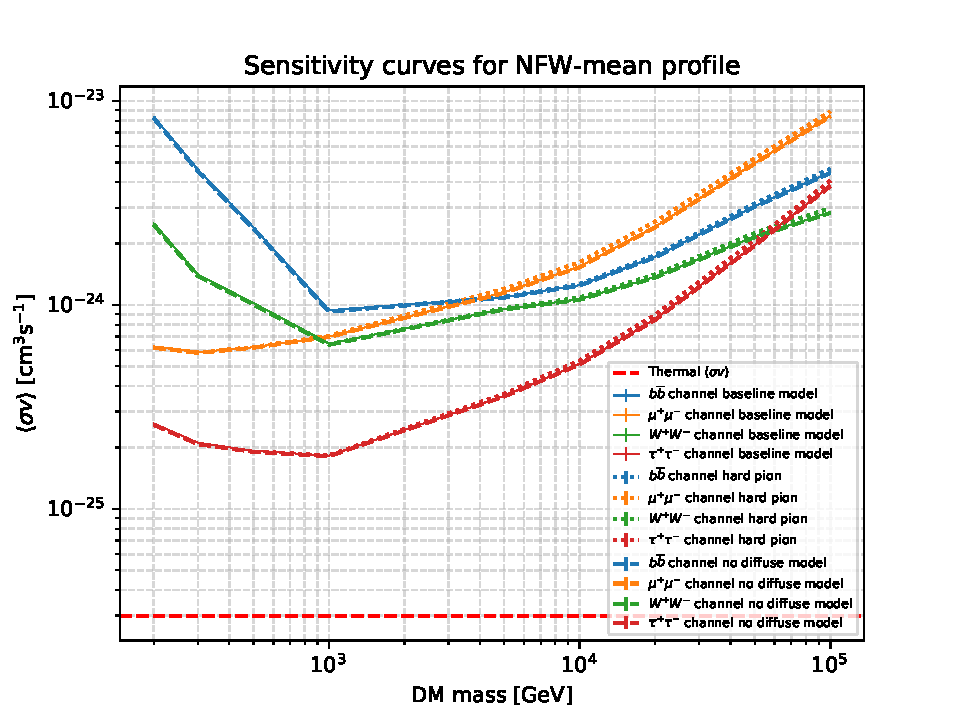
\includegraphics[width=1\textwidth]{Pictures/Limits_NFW-mean_comparediff.pdf}
  \endminipage
  \minipage{0.5\textwidth}
  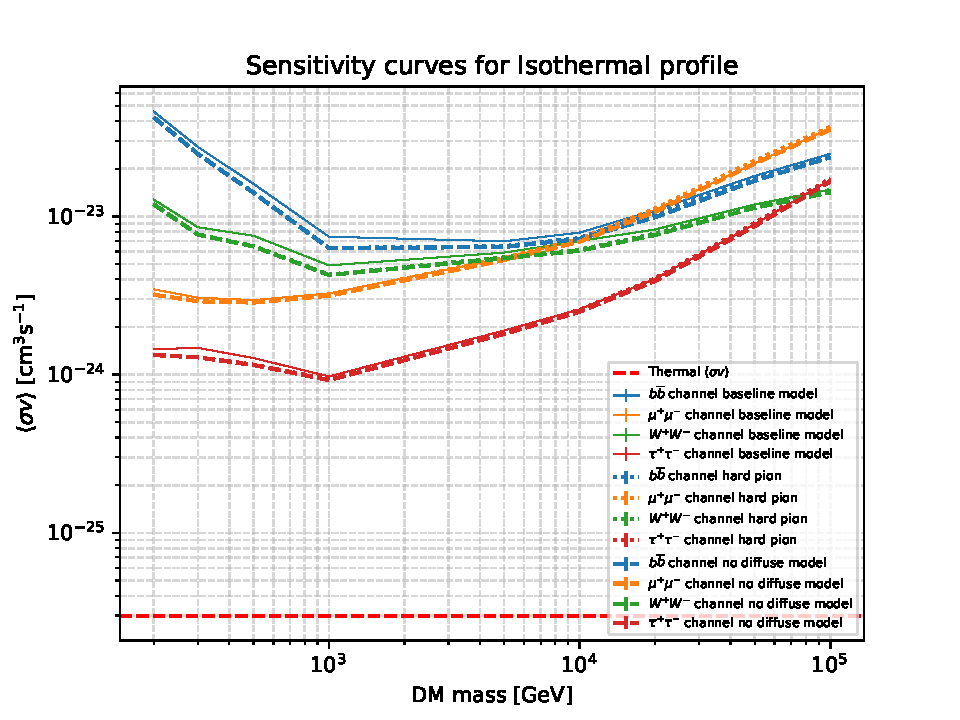
\includegraphics[width=1\textwidth]{Pictures/Limits_Isothermal_comparediff.pdf}
  \endminipage
  \caption{Sensitivity curves of $<\sigma v >$ vs. \gls{dm} particle mass for the NFW-mean (\textit{left}) and Isothermal-mean (\textit{right}) profiles for four annihilation channels, having three different cases of diffuse interstellar emission: Baseline model (thin line), no diffuse emission (dotted line) and pion decay emission with harder spectrum (dashed line).}
  \label{fig:dmsensi_diff}
  \end{figure}

\section{Summary and conclusions}

The deep survey of the \gls{lmc} will be an ambitious task which will account for many challenges, but that will potentially provide as many scientific results and new discoveries. Besides a lot of work can be done in the subject until \gls{cta} is fully available, in this work the first hints on the possible results of the survey have been studied.\\
Regarding the known point sources, a remarkable high significance has been obtained for all of them, meaning they will be easily detected within the survey with a binned likelihood analysis, which will allow to characterize the sources spectra in the \gls{cta} energy range, at least over 100 GeV. Given the duration of the survey (>300 h), it will also be possible to study the variability of LMC-P3, for which an upper flux limit for the off-peak emission has been derived. From the artificial population of \gls{pwne} introduced in the emission model, for 15 of them a significance sufficiently large to be detected has been obtained, providing an estimation of the number of new sources that \gls{cta} will be able to detect. The computed distribution of \gls{pwne} will serve as guide for a blind search, when dealing with real data from the survey.\\
One of the most interesting features of the \gls{lmc} is the fact that, as an extended source, it is possible to study the structure of its $\gamma$-ray emission, allowing to probe models of \gls{cr} injection and propagation. In this work, two models of diffuse emission of \gls{cr} due to leptonic \gls{ic} scattering and hadronic interactions leading to pion decay have been tested. The possibility to take into account the structure and distribution of \gls{cr} sources in the \gls{lmc} leads to the positive result on the detection of pion-decay emission following the model described in section \ref{sec:diffusemodel}. This is however a best-case scenario, where uncertainties in the model are not taken into account. It is still an encouraging result to make efforts on the refinement of the analysis and model computation of the diffuse emission in the \gls{lmc} for the future real data. The \gls{ic} component, on the other hand, has resulted in a too low significance, meaning it would be not possible to disentangle this emission component from the rest of the background. An upper flux limit has been derived for this model.\\
Finally, prospects on the detection of a possible $\gamma$-ray signal from \gls{dm} annihilation have been calculated. The results have established the parameter space of \gls{dm} models which will be possible to study with \gls{cta}. The main reasons to point towards the \gls{lmc} were its extended nature, which allow to rely on \gls{dm} spatial structure for its differentiation from the background and its relatively high J-factor, comparable to other popular \gls{dm} candidates such as \gls{dsphe}. However, the big population of other $\gamma$-ray emitters difficult the task of extracting a $\gamma$-ray signal coming from \gls{dm} annihilation. In the results presented in this thesis, several \gls{dm} profiles, annihilation channels and \gls{dm} particle masses have been tested on top of the emission model of the \gls{lmc}, to compute the velocity averaged annihilation cross section needed to detect the signal. It can be seen from picture \ref{fig:dmsensicurves}, that the majority of the models lie several orders of magnitude above the canonical thermal cross section, which is the self-annihilation cross section of \gls{wimp} \gls{dm} in the case of being a thermal relic. This result predicts that \gls{cta} will unlikely be able to exclude the canonical cross section for the typical \gls{wimp} \gls{dm} models, except for the most cuspy profiles (yet not very realistic) at \gls{dm} masses $\sim 1 TeV$ (case of nfw-cuspy profile and $\tau^+ \tau^-$ channel).\\
The work performed within this thesis will serve as a starting point for the future work that can be done regarding the \gls{lmc} \gls{ksp}. The emission model developed will serve as a benchmark for future studies and for the analysis of real data from the \gls{lmc} survey.
Other topics which have been left out of the scope of this thesis, but which still will benefit from its results could be a more detailed and realistic study on the possible new discovered sources, performing a totally blind search over the \gls{pwne} population as a more realistic analysis approach. The \gls{pwne} model can also be used to study the possibilities of detecting TeV halos in the \gls{lmc}, following a similar approach as \cite{2019tevhalos}. Other known sources, not yet detected in the \gls{vhe} range in the \gls{lmc}, such as \gls{snr} 1987A can be studied on top of the emission model to predict its detectability within the \gls{lmc} survey. Also, detailed studies on the spectral features which could be extracted from the detected sources can be performed, and many more science cases. On top of that, considering that the commissioning of \gls{cta} will take place in several phases, it sould be useful to perform a study of possible results obtained with a reduced number of telescopes (instead of the full array as has been done here).\\
The results presented in this chapter have been gathered in a \gls{cta} consortium paper currently in preparation phase, from which the author of this thesis is one of the corresponding authors.

\end{document}
 
